\documentclass[9pt,twocolumn,twoside,lineno]{gsag3jnl}
\usepackage{epstopdf}
\usepackage[utf8]{inputenc}
\articletype{inv} % article type
% {inv} Investigations
% {msr} Mutant Screen Reports
% {gs} Genomic Selection
% {goi} Genetics of Immunity
% {gos} Genetics of Sex
% {mp} Multiparental Populations

\runningtitle{Genome structure and molecular phylogeny of the only Eurasian \textit{Boechera} species, \textit{Boechera falcata} (Brassicaceae)} % For use in the footer

%% For the footnote.
%% Give the last name of the first author if only one author;
% \runningauthor{FirstAuthorLastname}
%% last names of both authors if there are two authors;
\runningauthor{Zilov and Mandáková \textit{et al.}}
%% last name of the first author followed by et al, if more than two authors.

\title{Genome structure and molecular phylogeny of the only Eurasian \textit{Boechera} species, \textit{Boechera falcata} (Brassicaceae)}

\author[$\dagger$,1, 2]{Danil Zilov}
\author[$\dagger$, $\ast\ast$, 3, 4]{Terezie Mandáková}
\author[5]{Marina Popova}
\author[6]{Michael D. Windham}
\author[$\ast$, 7, 8]{Vladimir Brukhin}

\affil[1]{Wellcome Sanger Institute, Wellcome Genome Campus, Hinxton, Cambridge, UK}
\affil[2]{ITMO University, Saint Petersburg, Russia}
\affil[3]{Central European Institute of Technology, Masaryk University, Czech Republic}
\affil[4]{Institute of Experimental Biology, Faculty of Science, Masaryk University, Czech Republic}
\affil[5]{Skolkovo Institute of Science and Technology, Moscow, Russia}
\affil[6]{Department of Biology, Duke University, Durham, U. S. A.}
\affil[7]{Department of Molecular, Biology and Biotechnology, School of Natural and Environmental Sciences, Newcastle University, UK}
\affil[8]{Lab of Embryology and Reproductive Biology, Komarov Botanical Institute, RAS, St. Petersburg, 2 Prof. Popov Str., Russia}

\correspondingauthoraffiliation[$\ast$]{Corresponding author: \href{mailto:vbrukhin@gmail.com}{vbrukhin@gmail.com} \\ \textsuperscript{\footnotesize $\ast\ast$}Co-correponding author: \href{mailto:terezie.mandakova@ceitec.muni.cz}{ terezie.mandakova@ceitec.muni.cz}}

\begin{abstract}

\textit{Boechera falcata} (Turcz.) Al-Shehbaz, previously known as \textit{Arabis turczaninowii} Ledeb., is a herbaceous perennial of the East Siberian, boreal-steppe ecotype. It is the sole species of the diverse genus \textit{Boechera} found on the Eurasian continent, with all other species endemic to North America and Greenland. Likely migrating from North America to Eastern Siberia via the Bering Land Bridge during the Pleistocene glaciation, \textit{B. falcata} presents a unique case for genomic study. The genus \textit{Boechera} is notable for its many allodiploid and triploid apomicts, which have arisen through complex hybridization of sexual species and ecotypes. To date, only the genomes of two American \textit{Boechera} species, \textit{B. stricta} and \textit{B. retrofracta}, have been sequenced and analyzed. In this study, we sequenced, assembled to the chromosome level, and analyzed the highly homozygous 189.36 Mb genome of \textit{B. falcata} (2n = 14). Molecular phylogenetic analysis of nuclear and organelle genomes revealed a high degree of relatedness to North American relatives. Cytogenetic analysis identified all 22 genomic blocks of crucifers, showing that five of the seven \textit{B. falcata} chromosomes are collinear with their ancestral counterparts, while two have undergone inversions. Allelic analysis of the apomixis marker APOLLO gene revealed that \textit{B. falcata} contains only sex alleles. The availability of the \textit{B. falcata} genome will advance studies of the evolution and phylogeny of Brassicaceae species and the mechanisms of apomixis, providing a crucial resource for future research in plant genetics and breeding.
\end{abstract}

\keywords{\textit{Boechera falcata}; Brassicaceae; genome structure; chromosome level genome assembly and annotation; chromosome rearrangements; comparative chromosome painting; molecular phylogeny; chloroplast genome}

\dates{\rec{xx xx, xxxx} \acc{xx xx, xxxx}}

\begin{document}

\maketitle
\thispagestyle{firststyle}
%\slugnote
\firstpagefootnote
\vspace{-13pt}% Only used for adjusting extra space in the left column of the first page
\equalcontrib{$\dagger$}

\section{Introduction}

The genus Boechera Á. Löve & D. Löve (Brassicaceae) comprises approximately 75 sexual diploid taxa and around 355 genetically distinct hybrid lineages, predominantly distributed in western North America \citep{alexander2013, hay2023}. \textit{Boechera falcata} (Turcz.) Al-Shehbaz, previously known as \textit{Arabis turczaninowii} Ledeb., is the sole species of this genus found in Eurasia, specifically endemic to Eastern Siberia and the Far East. Molecular marker data suggest that its origin may be linked to the migration of ancestral forms from North America to Siberia via the Bering Land Bridge \citep{al2005nomenclatural, windham2007, alexander2013, brukhin2019, kiefer2009phylogeographic}. 

Earlier classifications placed members of \textit{Boechera} within the genus \textit{Arabis} based on superficially similar morphological traits. However, karyological studies revealed chromosomal differences, prompting \cite{love1975nomenclatural} to separate the genus \textit{Arabis} (s.l.) into New World species with x = 7 (now classified as \textit{Boechera}) and Old World species with x = 8 (retained in \textit{Arabis}). Subsequent molecular phylogenetic analyses have confirmed that these two genera belong to distinct clades within the Brassicaceae \citep{koch1999, beilstein2010, nikolov2019, hendriks2023}, demonstrating that their similarities are convergent rather than indicative of a close evolutionary relationship.


Species of the genus \textit{Boechera} are closely related to the well-studied model plant \textit{Arabidopsis thaliana} within the Brassicaceae family. \textit{Boechera} is unique within this family for its documented apomixis \citep{moore1952cytological, bocher1969further,brukhin2019}. Apomixis is a form of asexual reproduction through seeds, where the embryo arises as a genetic clone of the maternal plant, developing parthenogenetically without the fusion of male and female germ cells. This ability to produce clones of a maternal plant and hence fix the desired genotypes in subsequent generations has significant potential for agricultural applications, facilitating effective plant breeding strategies \citep{grossniklaus2003engineering, bicknell2004, van2009apomixis, brukhin2017}. 

Diploid and triploid apomictic accessions of \textit{Boechera} exhibit signs of hybridogenic origin, leading changes in chromosome structure such as alloploidy, ascending dysploidy, substitution of homeologous chromosomes, and the appearance of aberrant extra chromosomes \citep{mandakova2016chromosome, brukhin2019}. Therefore, species from the genus Boechera serve as  unique models for molecular genetic studies of apomixis and the influence of hybridization of sexual forms on its occurrence.

A locus correlated with female apomeiosis, the \textit{APOmixis Linked Locus} (\textit{APOLLO}), has been identified, encoding an Asp-Glu-Asp-Asp-His exonuclease. Its expression is downregulated in sexual ovules as they enter meiosis and upregulated in apomeiotic ovules \citep{corral2013, bakin2022phylogenetic}. \textit{APOLLO} exhibits biallelic inheritance with both "apo-" and "sex-" alleles, differing by a 20-nucleotide polymorphism in the 5\textquotesingle{} untranslated region of the gene. All previously tested apomictic \textit{Boechera} accessions were heterozygous for \textit{APOLLO} alleles, having at least one apoallele and one sexallele, while all sexual accessions were homozygous for sexalleles \citep{corral2013, kliver2018, brukhin2019, bakin2022phylogenetic}. A high correlation (98.4\%) was observed between the presence of \textit{APOLLO} loci associated with apomixis and the apomictic mode of reproduction. The function of \textit{APOLLO} during reproduction in \textit{Boechera} remains unclear \citep{brukhin2019}. \cite{kliver2018} found two additional, more distant copies of \textit{APOLLO}, which may indicate past duplication events. It was shown that the apo- and sex alleles of \textit{APOLLO} arose after the separation of the genus \textit{Boechera}, forming two distint clades. An evolutionary scenario was proposed in which one of the \textit{APOLLO} copies could have acquired a new function in the common ancestor of \textit{Boechera}, leading to the separation of apomictic lineages. According to the Ka/Ks ratio = 1.4646 of \textit{APOLLO} alleles suggests that the branch leading to the apoalleles is under positive selection, typical for paralogs that have acquired a new function \citep{kliver2018, brukhin2019}.

To date, whole genome assemblies have been published for only two \textit{Boechera} species: \textit{B. stricta} \citep{lee2017young} and B. retrofracta \citep{kliver2018}. These species are of particular interest because, while they reproduce predominantly sexually, many of their hybrids are apomicts. The Far Eastern \textit{B. falcata} studied here is a key outgroup species for understanding the genome structure of the genus and the evolution of genetic loci associated with apomixis. This study aims to: 1) Achieve a chromosome-scale genome assembly of \textit{B. falcata}. 2) Perform a phylogenetic analysis to explore its relationship with North American \textit{Boechera} species. 3) Analyze genome structure, perform Hi-C genomic analysis , comparative genome analysis, and phylogenetic analysis based on nuclear and chloroplast DNA. 4) Study of the chromosome structure and evolution using comparative chromosome painting. 5) Study alleles of the apomixis-associated \textit{APOLLO} locus (encoding NEN exonuclease) in \textit{B. falcata} and add to the phylogenetic tree of \textit{APOLLO} locus isoforms of the \textit{Boechera} species published earlier \citep{kliver2018}.

\section{Materials and methods}
\label{sec:materials:methods}

\subsection{Plant Material}
Seeds of \textit{B. falcata} were collected from plants (Figure \ref{fig:plant}) in natural habitats: a petrophytic open community of \textit{Artemisia gmelinii} Weber ex Stechm. and \textit{B. falcata} on the southern slope with a steepness of 45º (Tenkinsky district of the Magadan region, 10 km southeast of the village of Orotuk, Russia - 62º 01'50.586" N, 148º 38'46.591" E). 
Plants were cultivated from seeds in the greenhouse of CEITEC Masaryk University under the standard conditions (16/8 h light/dark, 21/18 °C, 15 µmol/m2/s). Specimens are deposited at the Herbarium of Masaryk University (BRNU): BRNU sheet numbers: 696364 (\url{https://brnu.jacq.org/BRNU696264}) and 696267 (\url{https://brnu.jacq.org/BRNU696267}) (Suppl. Figure 1).

\begin{figure}[t!]
\renewcommand{\familydefault}{\sfdefault}\normalfont
\centering
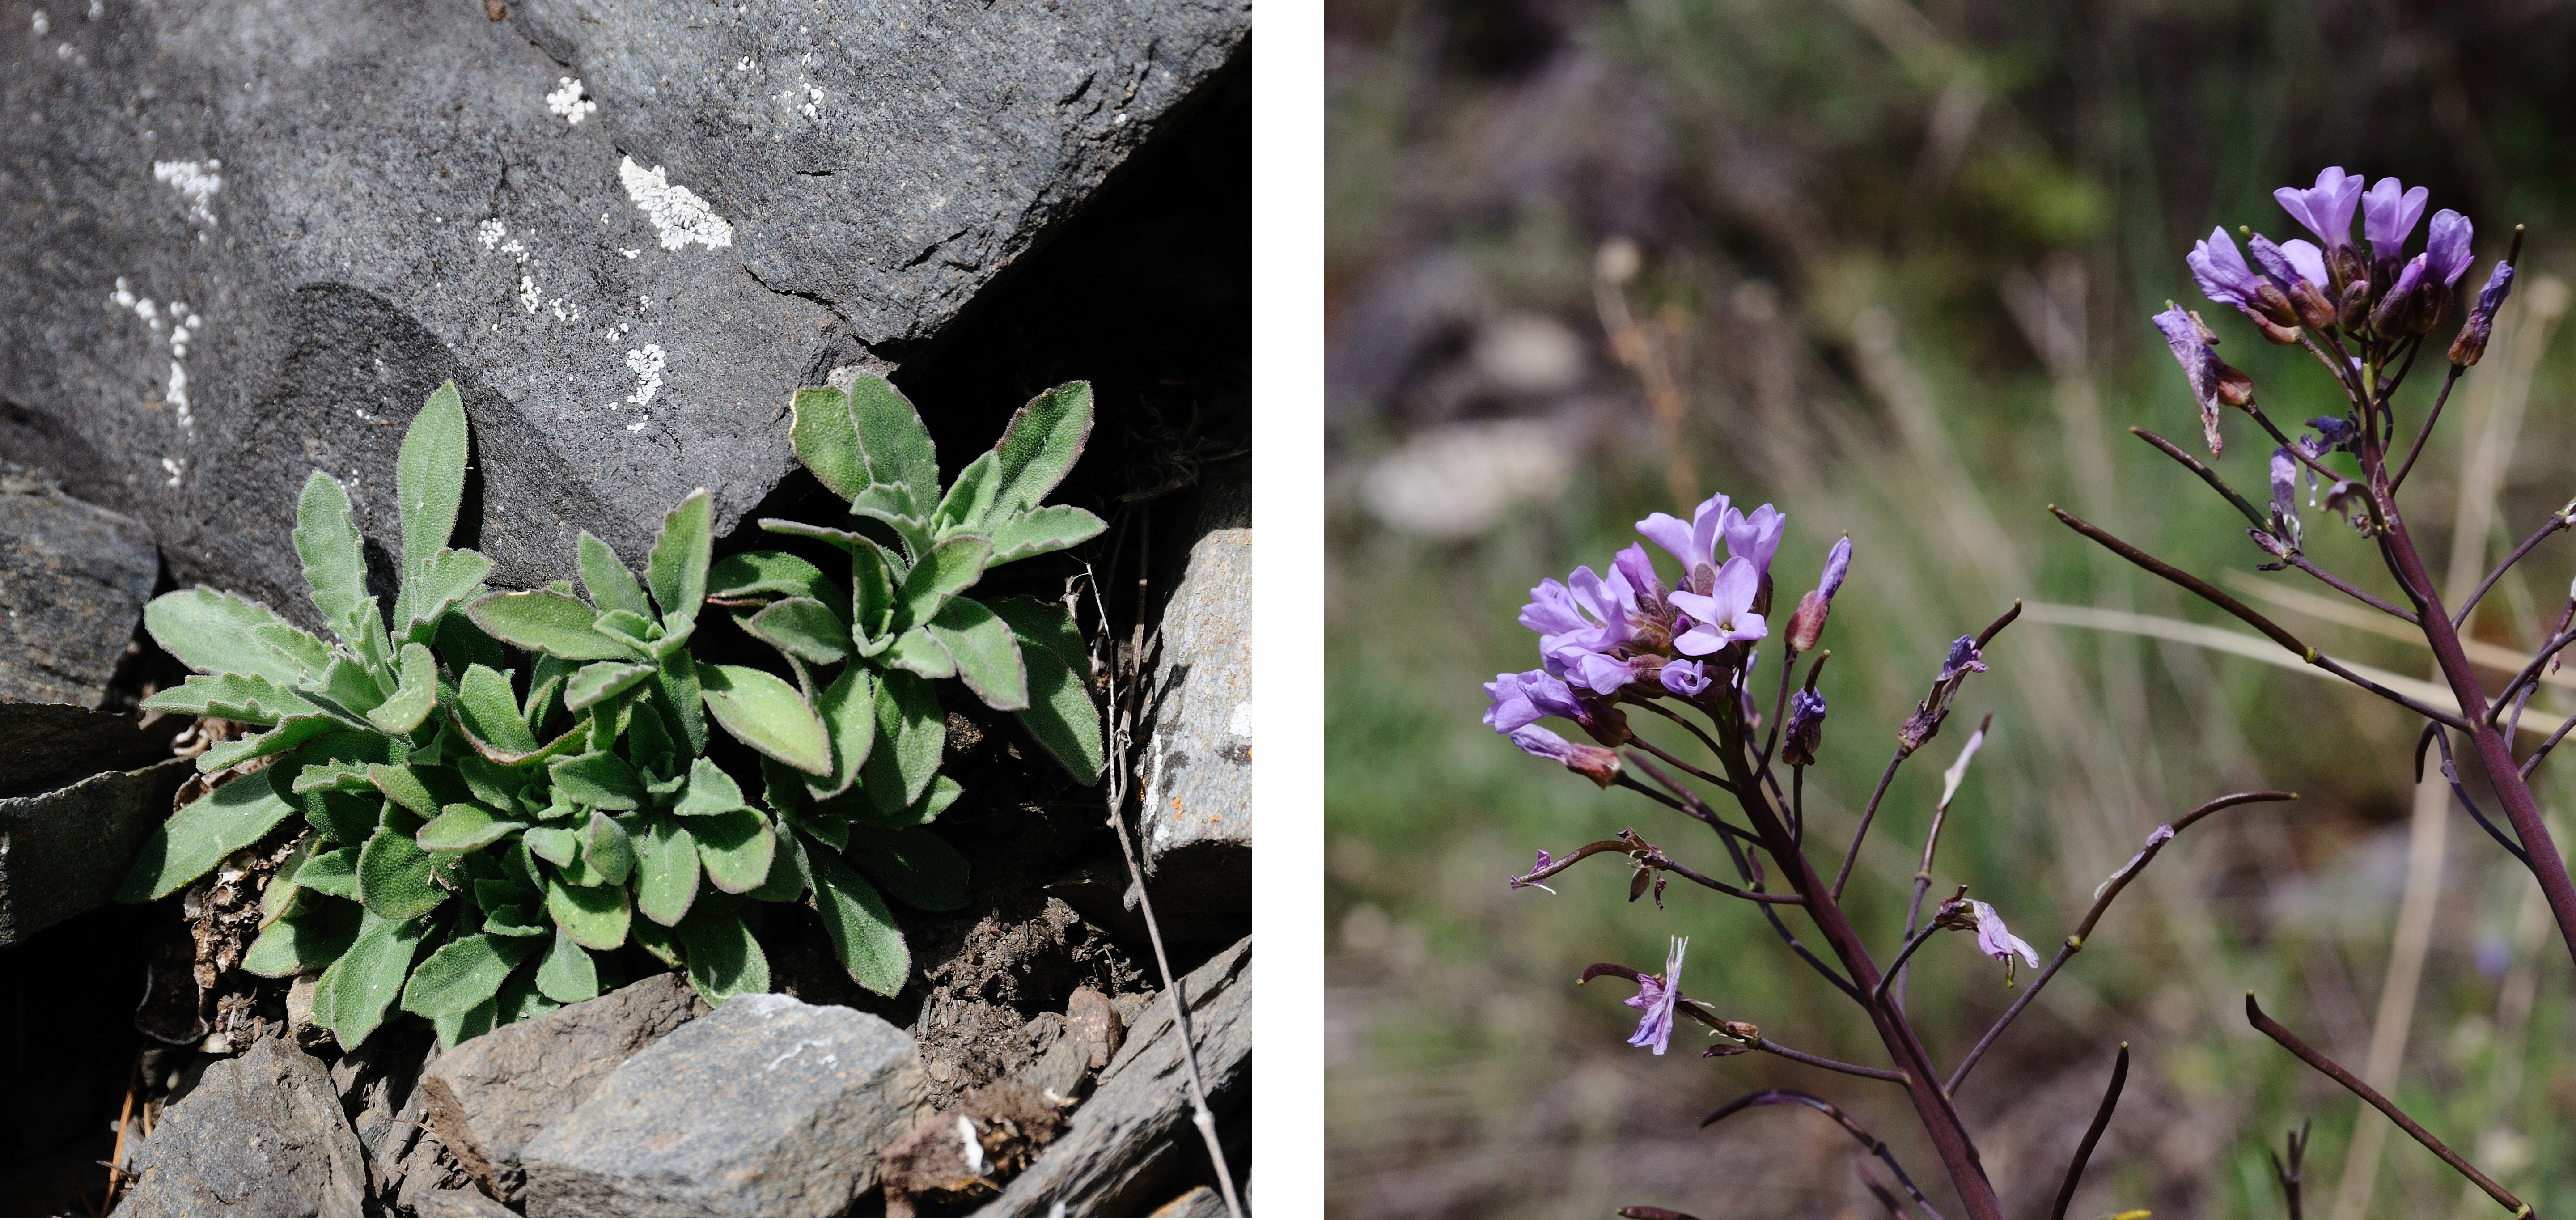
\includegraphics[width=\linewidth]{figures/falcata_photo.jpg}
\caption{Plants of \textit{Boechera falcata} (leave rosette and blooming plants with siliques) growing in the Kolyma River valley in the Magadan region, from which seeds were collected.}
\label{fig:plant}
\end{figure}

\subsection{Microsatellite genotyping}

Genomic DNA was extracted using the Qiagen DNeasy Plant Mini Kit. Microsatellite allele variation was assessed at 15 previously published loci (A1, A3, B6, Bdru266, BF3, BF9, BF11, BF15, BF18, BF19, BF20, C8, E9, ICE3, ICE14) following \cite{beck2012}. Forward primers for each locus were labeled with either 6-FAM or HEX. Multiplex polymerase chain reaction (PCR) was performed for sets of three loci simultaneously. Each \( 50 \, \mu\text{l} \) reaction contained \( 15 \, \mu\text{l} \) of \( 2\times \) Qiagen Multiplex PCR Master Mix, \( 3 \, \mu\text{M} \) of the primer set, and approximately 40 ng of gDNA template. The PCR conditions included an initial denaturation at \( 95^\circ\text{C} \) for 15 min, followed by 30 cycles of denaturation at \( 95^\circ\text{C} \) for 30 s, annealing at \( 53^\circ\text{C} \) for 90 s, and extension at \( 72^\circ\text{C} \) for 60 s, with a final extension step at \( 60^\circ\text{C} \) for 30 min. PCR products were first analyzed on a 1--3\% agarose gel. Capillary electrophoresis was then performed by Macrogen using a 400HD standard. Electropherograms were analyzed with the Microsatellite plugin of Geneious software, and species identity was determined using the \textit{Boechera} Microsatellite Website \url{https://windhamlab.biology.duke.edu/} \citep{li2017}.

\subsection{Chromosome preparation and comparative chromosome painting}

Mitotic and meiotic (pachytene) chromosome preparations were performed according to the protocol outlined by \cite{mandakova2016chromosome}. Before analysis, suitable slides were pre-treated with RNase (100 mg/ml) and pepsin (0.1 mg/ml). Comparative chromosome painting was performed according to \cite{mandakova2020chromosomal}. Fluorescent signals were examined and captured using a Zeiss Axioimager epifluorescence microscope equipped with a CoolCube camera (MetaSystems). Images were acquired separately for each of the four fluorochromes using their respective excitation and emission filters (AHF Analysentechnik). The collected images were then pseudocolored and merged using Adobe Photoshop CS6 (Adobe Systems).

\subsection{Whole Genome Sequencing Strategy}

\subsubsection{DNA extraction and prob preparation}

DNA was extracted following \cite{huang2023} protocol. The \textit{B. falcata} genome was sequenced on the three WGS platforms: Illumina NovaSeq with 150bp PE sequencing run, final 75Gb data obtained, with 243x coverage; Pacbio sequel II (HiFi/CCS mode/cell) (1 SMRT cell), genome coverage - 129x; Hi-C genomic analysis technique ~50M Read-Pairs, genome coverage - 30x.

\subsubsection{Raw Data Filtration and Pre-Processing}
Raw Illumina reads and HiC reads trimming were processed using Trimmomatic v0.32 \citep{bolger2014} with the following parameters ILLUMINACLIP:2:30:10:2:True LEADING:3 TRAILING:3 MINLEN:36. HiFi reads evaluation of length and quality stats was performed with pauvre tool \url{https://github.com/conchoecia/pauvre}.
The quality assessment of HiFi reads using the Pauvre tool indicated a mean read length of 13,387 bases and an N50 value of 13,975 bases. The Phred quality scores ranged from 20 to 50, with a peak at 40 (Suppl. Figure 2).



\subsubsection{Genome Coverage Estimation}
Estimation of the genome coverage based on the 23-mer distribution and k-mer based statistics was performed using the a genomic k-mer counter Meryl (\url{https://github.com/marbl/meryl}), k-mer databases of HiFi and Illumina WGS reads, and GenomeScope2 \cite{ranallo2020genomescope}.


\subsection{Genome Assembly and Quality Control}

For genome assembly we performed a bake off with four different assemblers: for HiFi reads: flye v2.9.2-b1786 \citep{kolmogorov2019}, verkko v1.4.1 \citep{rautiainen2023}, nextdenovo 2.5.2 \citep{hu2024nextdenovo}, and hifiasm v0.19.6-r595 \citep{cheng2021} (Table \ref{tab:genome_assemlby_stats}). Flye was run with the --keep-haplotypes option, while verkko and nextdenovo targeted a genome size of 200Mbp. Nextdenovo and hifiasm were executed with standard parameters for HiFi reads. The assembly process was automated using the hifiblender pipeline \url{https://github.com/zilov/hifiblender}.
Quality of the assembly was assessed using multiple metrics: N50, L50, BUSCO completeness, and QV (Quality Value). QUAST \citep{gurevich2013} was utilized for contiguity statistics, BUSCO \citep{seppey2019busco} for completeness assessment, and Merfin \citep{formenti2022} for QV (Quality Value) calculation using a Meryl HiFi + Illumina hybrid k-mer database (k=23). Coverage of the genome was calculated with GenomeScope2 \cite{ranallo2020genomescope}. 
Haplotype phasing was performed using hapdup \url{https://github.com/KolmogorovLab/hapdup} with default parameters. Polishing was conducted with nextpolish \citep{hu2020} using Illumina reads, with the number of steps (three for the first pseudo-haplotype, two for the second) determined by QV value progression checked on hybrid HiFi and Illumina Meryl database.
Scaffolding and genome curation Hi-C was facilitated by yahs \citep{zhou2023yahs}, followed by genome curation using juicebox \citep{durand2016juicebox}. The hic-scaffolder pipeline \url{https://github.com/zilov/hic-scaffolder} streamlined Hi-C read alignment and scaffolding processes. Finally, we aligned the orientation and order of chromosomes to match the \textit{Boechera} stricta assembly (NCBI GenBank assembly ID: GCA\_018361395.1).

\subsection{Organelle DNA Assembly and Annotation}
Mitochondrial and chloroplast genomes were assembled using contigs from the whole genome assembly after polishing and HiC scaffolding steps. For the mitochondrial genome, we employed MitoHiFi \citep{uliano2023mitohifi}, using the \textit{B. stricta} mitochondrion as a reference to identify and assemble a complete circular mitochondrial sequence.
The chloroplast genome assembly required additional manual steps. While MitoHiFi software typically assembles circular organelle genomes, it failed to automatically reconstruct the complete circular chloroplast genome in our case. Therefore, we developed an alternative approach. First, we used the \textit{B. stricta} chloroplast genome as a reference to identify chloroplast-derived contigs. Then, we performed BLAST analysis to find overlapping regions between these contigs. Using these overlapping sequences, we manually constructed the complete circular chloroplast genome.
Chloroplast and mitochondrial genome annotation and visualization were performed using GeSeq \citep{tillich2017} and manually curated by OGDRAW 
\cite{greiner2019}, respectively.

\subsection{Nuclear Genome Annotation}

To call for repetitive elements in the genome we used EarlGrey \citep{baril2024earl} repeat masking pipeline. A custom repeat database was created by combining the PlantRep database \citep{luo2022} and the nrTEplants dataset \citep{contreras2021k}. Initial masking was conducted with the "eukarya" search term. De novo repeat identification performed with RepeatModeler \citep{flynn2020repeatmodeler2}. The custom database was then used for subsequent rounds of masking to ensure identification of repetitive elements specific to plant genomes. EarlGrey utilizes a combination of tools, including RepeatModeler \citep{flynn2020repeatmodeler2}, RepeatMasker
\url{https://repeatmasker.org/}, LTR\_FINDER \citep{xu2007}, and others to refine and cluster repeat sequences.
For coding gene annotation, we employed BRAKER v3.0.8 \citep{gabriel2024braker3} in compleasm \citep{huang2023} mode, utilizing the Viridiplantae OrthoDB \citep{kriventseva2019} protein database for homology-based prediction.

\subsection{Comparative analysis of \textit{Boechera falcata} and \textit{Boechera} stricta genomes}

We compared the assembled genome of \textit{B. falcata} with the published \textit{Boechera stricta} genome (NCBI GenBank assembly ID: GCA\_018361395.1). Both genomes were evaluated using QUAST and BUSCO. QV calculations were performed differently: for \textit{B. falcata} , k-mer analysis was carried out based on the hybrid HiFi and Illumina reads (\url{https://github.com/arangrhie/T2T-Polish/tree/master/merqury}), while for \textit{B. stricta} k-mer analysis performed using only Nanopore reads due to their availability. Repeat masking and annotation were performed on both genomes. Synteny analysis between \textit{B. falcata} and \textit{B. stricta} chromosomes was conducted using SyRI \citep{goel2019syri}. Whole-genome alignment visualization was generated with the help of D-GENIES \citep{cabanettes2018} to produce a comparative dotplot.

\subsection{Phylogenetic Analysis of \textit{B. falcata} Among the Other \textit{Boechera} and Brassicaceae Species.}

The phylogenetic analysis of \textit{B. falcata} was conducted in the context of other \textit{Boechera} and Brassicaceae species using a combination of Angiosperms353 and Brassicaceae764 probe sets, following a methodology similar to that described by \citep{hay2023}. Loci were assembled using HybPiper version 2.1.7 \citep{johnson2016hybpiper} with Illumina reads. Assembled loci were added to the existing locus files of other \textit{Boechera} species. Each locus was aligned using MAFFT \citep{katoh2008} with the L-INS-I method. Alignments were concatenated into a supermatrix using FASconCAT-G \citep{kuck2014fasconcat} and subsequently trimmed using trimAl \citep{capella2009trimal} with the -automated1 setting to reduce gaps and missing data. Phylogenetic tree construction was performed using RAxML-NG v1.2.0 \citep{kozlov2019raxml}, employing the GTR+F+R model and generating 1000 bootstrap replicates.

To analyze the phylogeny based on the chloroplast genome, we extracted 47 chloroplasts genes (listed in Suppl. Table 1) from the complete chloroplast assemblies of \textit{Boechera} species and other Brassicaceae species reported elsewhere \citep{zhu2021}. Phylogenetic analysis of chloroplast genomes was performed in MEGA (v.11.0.10) \citep{tamura2007mega4}: ClustalW(Codons) option with default settings was used for alignment of gene sequences. Phylogenetic tree was constructed with the Neighbor-Joining test with bootstrap 1000.

\subsection{Analysis of \textit{APOLLO} Sex- and Apo-alleles in \textit{B. falcata} Genome.}

The \textit{APOLLO} gene \citep{corral2013} was identified in the annotated genome using BLAST search. Additional gene sequences for phylogenetic analysis were obtained from \cite{bakin2022phylogenetic}. Multiple sequence alignment was performed using MUSCLE \citep{edgar2004}. Phylogenetic tree construction was carried out with RAxML-NG v1.2.0 \citep{kozlov2019raxml}, employing the following parameters: -all -model JTT+G --bs-trees 1000 --tree pars{10}.

\subsection{Visualization}

Visualization of HiC-plot was performed with cooler \url{https://github.com/open2c/cooler}, with each point on the plot representing 80kbp. Circos plot was built with pyCirclize \url{https://github.com/moshi4/pyCirclize}. The phylogenetic trees were visualized with iTol \citep{letunic2021}. The synteny plots were built with plotsr \citep{goel2022plotsr}, dotplot of genome to genome alignment with dgenies \citep{cabanettes2018}.

\section{Results and discussion}

\subsection{Chromosome count}

Chromosome number was determined from young anthers of ten plants cultivated from seeds, confirmed by microsatellite genotyping as \textit{B. falcata} . All plants were confirmed to be diploid, with a chromosome count of \( 2n = 14 \) (Figure \ref{fig:karyotype}).

\subsection{Karyotype structure}

Bacterial artificial chromosome-based comparative chromosome painting was employed to investigate the genome structure of \textit{B. falcata} . Probes were arranged according to the ancestral Boechereae genome structure \citep{mandakova2020chromosomal}, allowing the mapping of all 22 crucifer genomic blocks \citep{mandakova2019origin} onto \textit{B. falcata} chromosomes (BoeFa1–BoeFa7) (Figure \ref{fig:karyotype}; \ref{fig:ancestral-chromosomes}). Notably, five of the seven \textit{B. falcata} chromosomes (BoeFa1, BoeFa2, BoeFa4, BoeFa5, BoeFa7) exhibit collinearity with their corresponding chromosomes in the ancestral Boechereae genome \citep{mandakova2020chromosomal}. In contrast, BoeFa3 contains a pericentric inversion involving genomic block W, while BoeFa6 undergoes a paracentric inversion within its short arm, with breakpoints located within genomic blocks O and P (Figure \ref{fig:karyotype}; \ref{fig:ancestral-chromosomes}).

\begin{figure}[t!]
\renewcommand{\familydefault}{\sfdefault}\normalfont
\centering
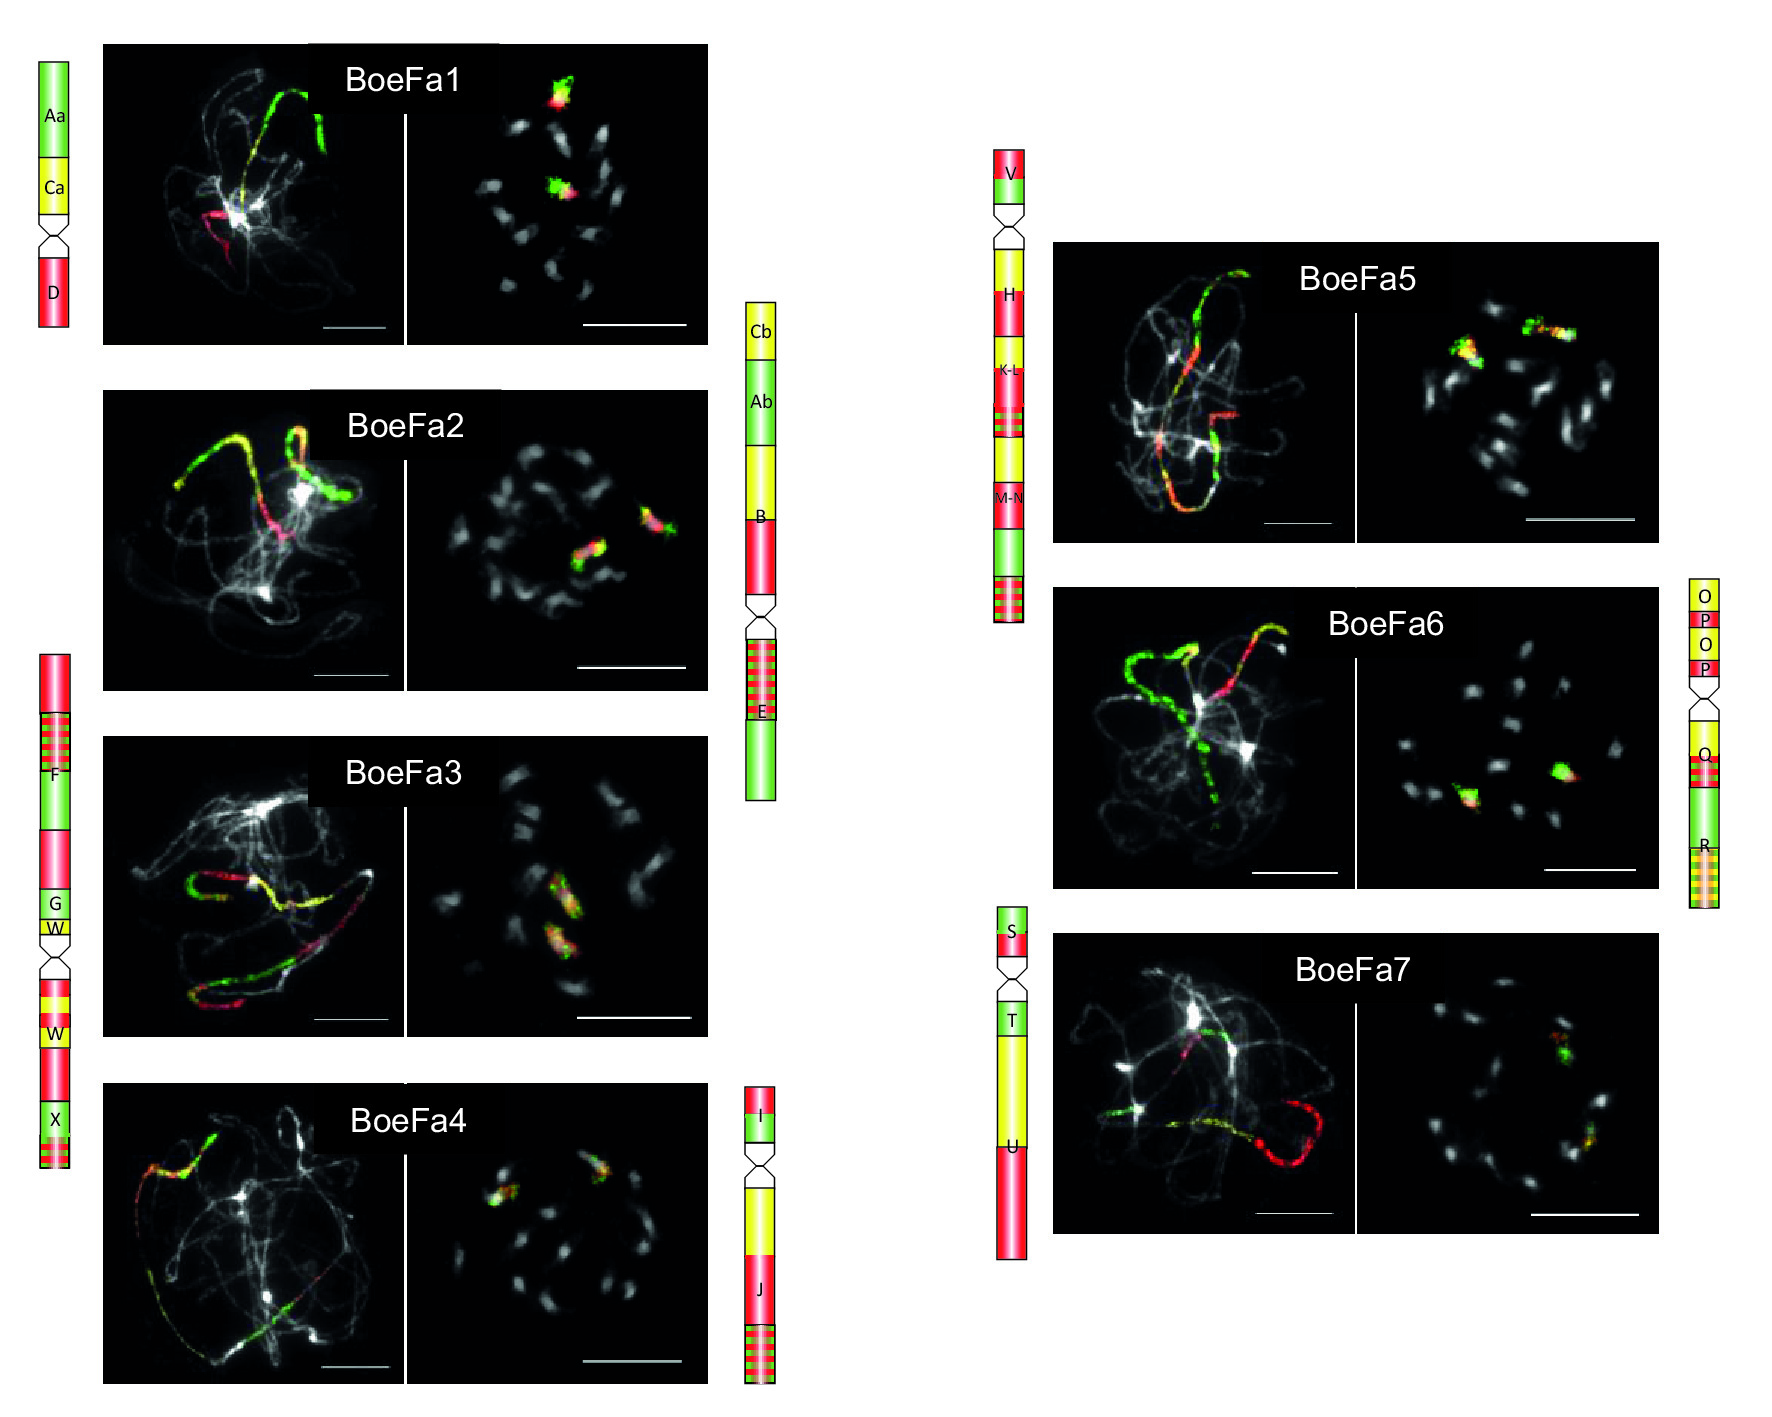
\includegraphics[width=\linewidth]{figures/Figure 2.jpg}
\caption{Karyotype structure of \textit{B. falcata} inferred from comparative chromosome painting (CCP). The seven chromosomes (BoeFa1–BoeFa7) were visualized through CCP using\textit{Arabidopsis} BAC contigs as painting probes applied to pachytene, mitotic, and diakinesis chromosome spreads. Painting signals are shown in experimental colors, reflecting the fluorochrome(s) used to label specific genomic blocks (GBs). All chromosomes were counterstained with DAPI and presented as grayscale images. Scale bars, \( 10 \ \mu\text{m} \).}
\label{fig:karyotype}
\end{figure}

\begin{figure}[t!]
\renewcommand{\familydefault}{\sfdefault}\normalfont
\centering
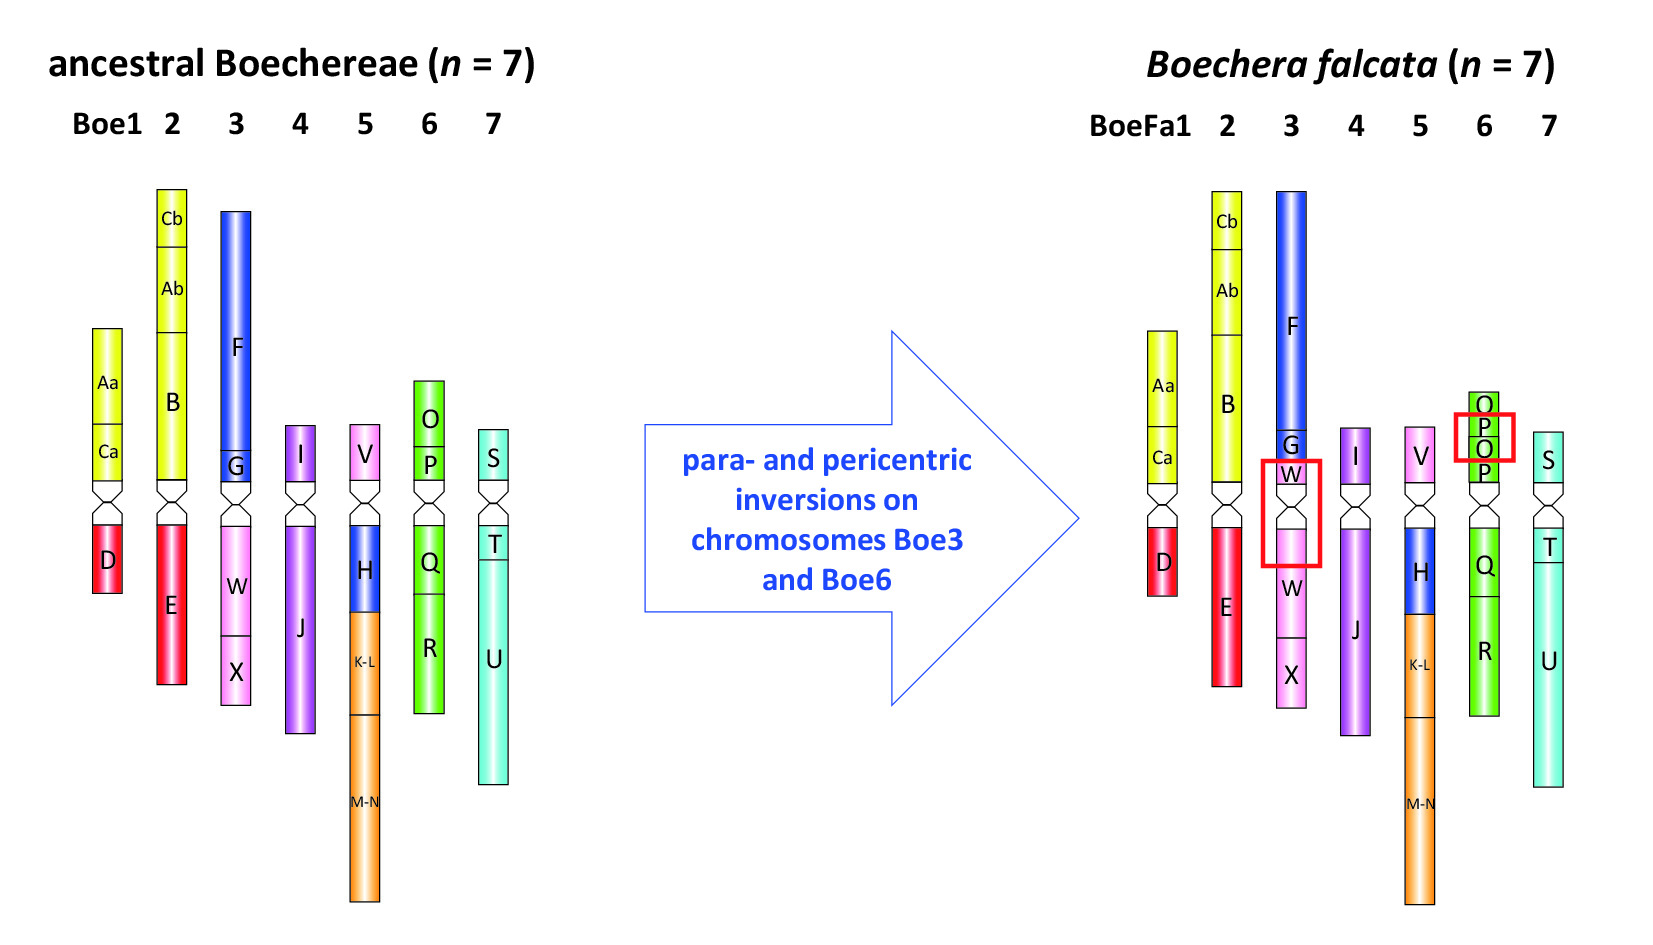
\includegraphics[width=\linewidth]{figures/Figure 3.jpg}
\caption{Chromosome evolution of \textit{B. falcata} from the ancestral Boechereae genome \citep{mandakova2020chromosomal}. Color coding of 22 genomic blocks (GBs, A to X) reflects their position on the eight ancestral chromosomes in the Ancestral Crucifer Karyotype \citep{lysak2016comparative}. The ideograms are drawn to scale, whereby the size of GBs corresponds to the size of homeologous blocks in the Arabidopsis thaliana genome (The Arabidopsis Information Resource, TAIR; \url{http://www.arabidopsis.org}.}
\label{fig:ancestral-chromosomes}
\end{figure}

\subsection{k-mer Based Statistics Indicates a High Level of \textit{B. falcata} Genome Homozygosity}

k-mer spectrum built by GenomeScope2 software \citep{ranallo2020genomescope} for both Illumina and HiFi reads is shown in Figure \ref{fig:genomescope}. The 23-mer distribution has one major peak at 249\(\times\) coverage corresponding to diploid 23-mers (shared between homologous chromosomes), also small heterozygous peaks (122\(\times\) and 64\(\times\)) were detected (Figure \ref{fig:genomescope}). According to the assessment, the genome was highly homozygous with 99,9\% of AA k-mers for both Illumina and HiFi reads. The genome size of \textit{B. falcata} was estimated to be close to 185 Mbp by Illumina k-mers and 219 Mbp by HiFi k-mers, which is in the range of the previous estimations of a minimal genome size of \(\sim\)200 Mbp in \textit{Boechera} \citep{anderson2011}. Homozygosity of genomes in \textit{Boechera} is characteristic of sexual reproduction, since all apomicts studied are usually heterozygous, allodiploids or polyploids \citep{brukhin2019}. Sexuality in \textit{B. falcata} was also confirmed by cytoembryological studies \citep{vinogradova2023development}.

\begin{figure}[t!]
\renewcommand{\familydefault}{\sfdefault}\normalfont
\centering
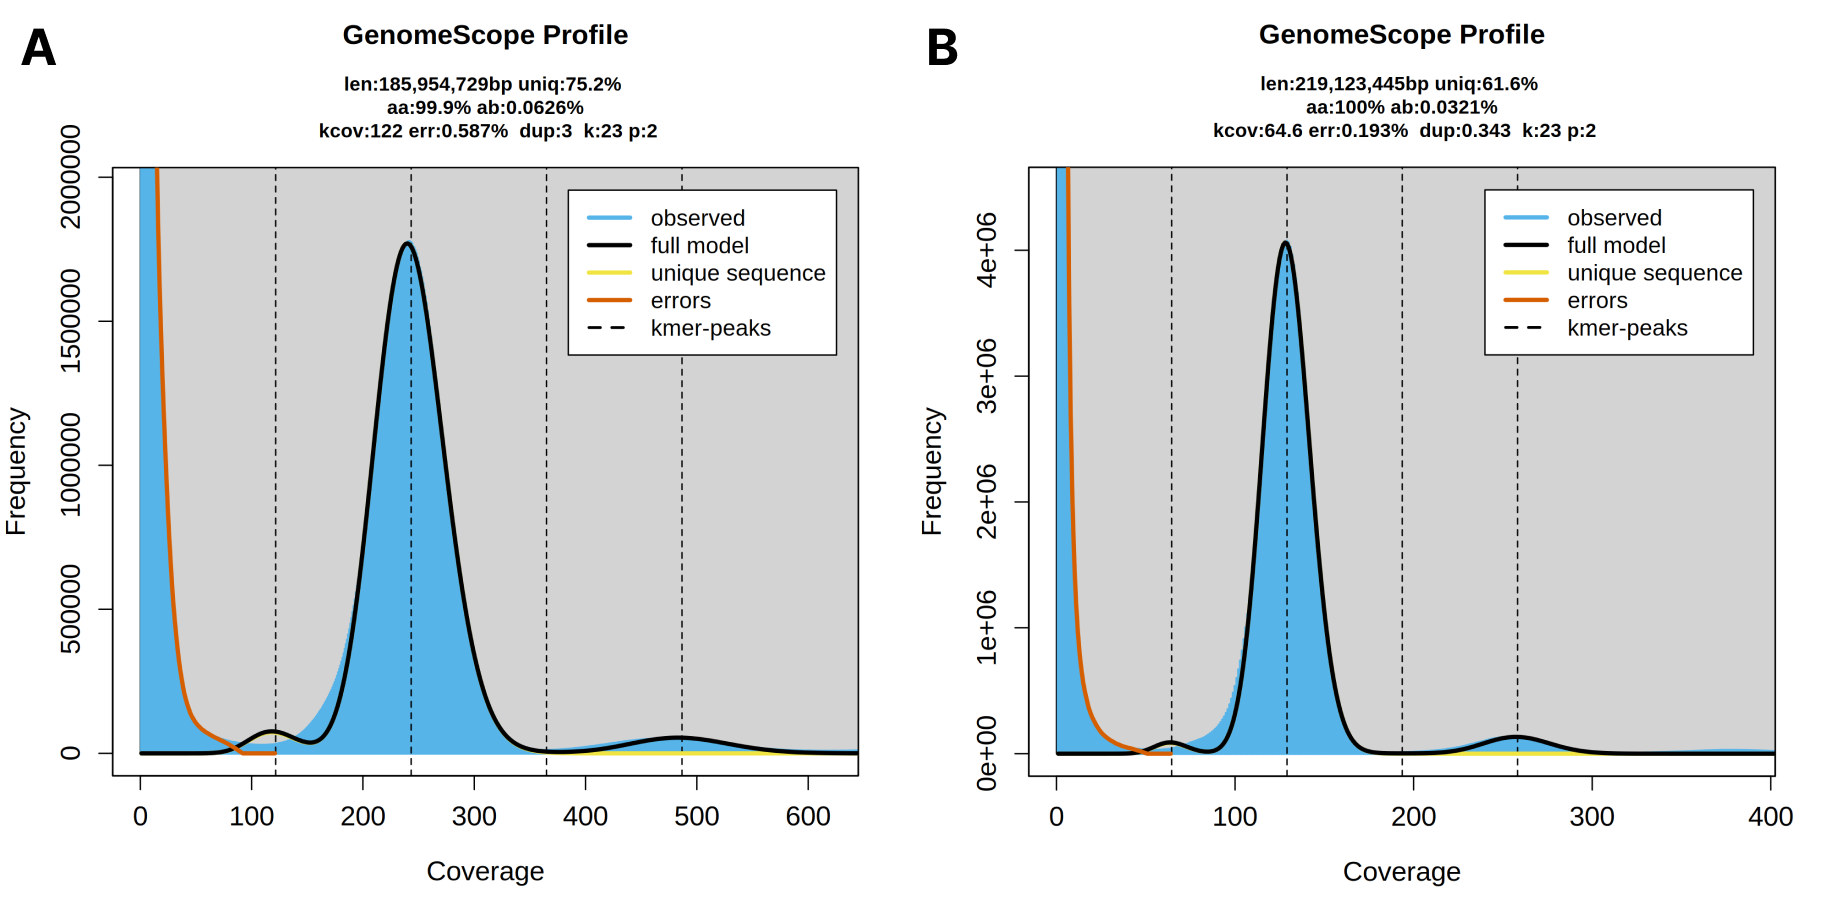
\includegraphics[width=\linewidth]{figures/genomescope_illumina_hifi.png}
\caption{Distribution of 23-mers for detection genome size and evaluation of homo/heterozygosity (A) for Illumina PE reads and (B) HiFi libraries. Only one major peak is present in both Illumina (at 249x coverage) and HiFi (129x) libraries.}
\label{fig:genomescope}
\end{figure}


\subsection{Assessment of the Quality of Genome Assembly Performed by Different Assemblers}

To identify the most efficient and correct \textit{Boechera falcata} genome construction, we compared four different assemblers: NextDenovo, flye, hifiasm, and verkko (Table \ref{tab:genome_assemlby_stats}). The assemblies varied considerably in their contiguity and quality metrics. NextDenovo assembler demonstrated the highest contiguity with only 50 contigs achieving N50 of 12,407,843 bp, L50 of 7. Evaluation of the assembly completeness was performed using BUSCO, complete BUSCO score is 98.8\% (95.8\% single-copy, 3.0\% duplicated). This assembly also exhibited the highest Merqury QV (62.83) and Merfin QV* (32.99) scores, indicating greater accuracy compared to the other assemblies.
The hifiasm assembler produced the most contigs (1232) and achieved the highest N50 value of 30,472,172 bp. However, it showed a higher number of overrepresented k-mers and lower QV scores compared to the NextDenovo and flye assemblers.
In fact, all assemblies showed complete BUSCO genes ($\geq$ 98. 7\%), indicating a high completeness of the assembly under different assembly strategies. The GC content was similar in all assemblies and ranged from 35.95\% to 37.85\%. However, based on the obtained metrics, we chose the NextDenovo assembler for further haplotype phasing, polishing, analysis, and improvement of the Hi-C scaffolding due to its favorable balance of continuity, completeness, and accuracy.

\begin{table*}[p]
\centering
\caption{Comparative statistics of genome assembly by different assemblers}
\begin{tableminipage}{\textwidth}
\begin{tabularx}{\textwidth}{@{}XXXXX@{}}
\hline
\textbf{}                             & \textbf{NextDenovo}                                   & \textbf{flye}                                         & \textbf{hifiasm}                                      & \textbf{verkko}                                       \\
\hline
Contigs №                             & 50                                                    & 145                                                   & 1232                                                  & 2041                                                  \\
Total length (bp)                     & 189363209                                             & 201258247                                             & 249420951                                             & 246125585                                             \\
GC (\%)                               & 35.95                                                 & 35.96                                                 & 36.53                                                 & 37.85                                                 \\
N50                                   & 12407843                                              & 6341302                                               & 30472172                                              & 7370569                                               \\
L50                                   & 7                                                     & 11                                                    & 4                                                     & 11                                                    \\
K-mers not found in reads (missing)   & 1929                                                  & 2859                                                  & 21778                                                 & 75086                                                 \\
K-mers overly represented in assembly & 1460638                                               & 3908427                                               & 31538183                                              & 27968096                                              \\
Merqury QV                            & 62.83                                                 & 62.09                                                 & 46.84                                                 & 47.36                                                 \\
Merfin QV*                            & 32.99                                                 & 30.69                                                 & 24.05                                                 & 23.71                                                 \\
Total low-coverage regions:           & 0                                                     & 0                                                     & 0                                                     & 0                                                     \\
BUSCO                                 & C:98.8\%{[}S:95.8\%,D:3.0\%{]}, F:0.2\%,M:1.0\%,n:4596 & C:98.8\%{[}S:95.7\%,D:3.1\%{]}, F:0.2\%,M:1.0\%,n:4596 & C:98.8\%{[}S:95.9\%,D:2.9\%{]}, F:0.2\%,M:1.0\%,n:4596 & C:98.7\%{[}S:95.6\%,D:3.1\%{]}, F:0.2\%,M:1.1\%,n:4596 \\
\hline
\end{tabularx}
  \label{tab:genome_assemlby_stats}
\end{tableminipage}
\end{table*}

\subsection{Genome Polishing}

After splitting haplotypes to dual assembly with hapdup, both primary and alternate haplotype underwent three rounds of polishing using Illumina reads (Table \ref{tab:genome_polishing_stats}). Each polishing step progressively improved the assembly quality, as evidenced by the decreasing number of missed k-mers and increasing Merqury QV scores. After the final polishing step, the primary haplotype achieved a Merqury QV of 68.04, while the alternative haplotype reached 67.6, indicating high accuracy in both haplotypes.

\begin{table*}[p]
\centering
\caption{Genome polishing statistics}
\begin{tableminipage}{\textwidth}
\begin{tabularx}{\textwidth}{CCC}
\hline
\textbf{Polishing step} & \textbf{Primary haplotype missed kmers/Merqury QV} & \textbf{Alternative haplotype missed kmers/Merqury QV} \\
\hline
Step 1                  & 893 / 66.88                                        & 1020 / 66.3                                            \\
Step 2                  & 837 / 67.16                                        & 732 / 67.74                                            \\
Step 3                  & 683 / 68.04                                        & 757 / 67.6\\                                       
\hline
\end{tabularx}
  \label{tab:genome_polishing_stats}
\end{tableminipage}
\end{table*}

\subsection{Hi-C Scaffolding and Chromosome-Level Assembly}

Following genome assembly, haplotype phasing, and polishing, we performed Hi-C scaffolding to achieve a chromosome-level assembly. This process resulted in the successful construction of 7 chromosomes, consistent with the known karyotype of \textit{Boechera} species (Fig. \ref{fig:hic-and-genome}). The final assembly contained a total of 32 gaps. The assemblies of the primary and alternate haplotypes are available on the NCBI, BioProjects: PRJNA1077252 and PRJNA1100512, respectively.

\begin{figure}[t!]
\renewcommand{\familydefault}{\sfdefault}\normalfont
\centering
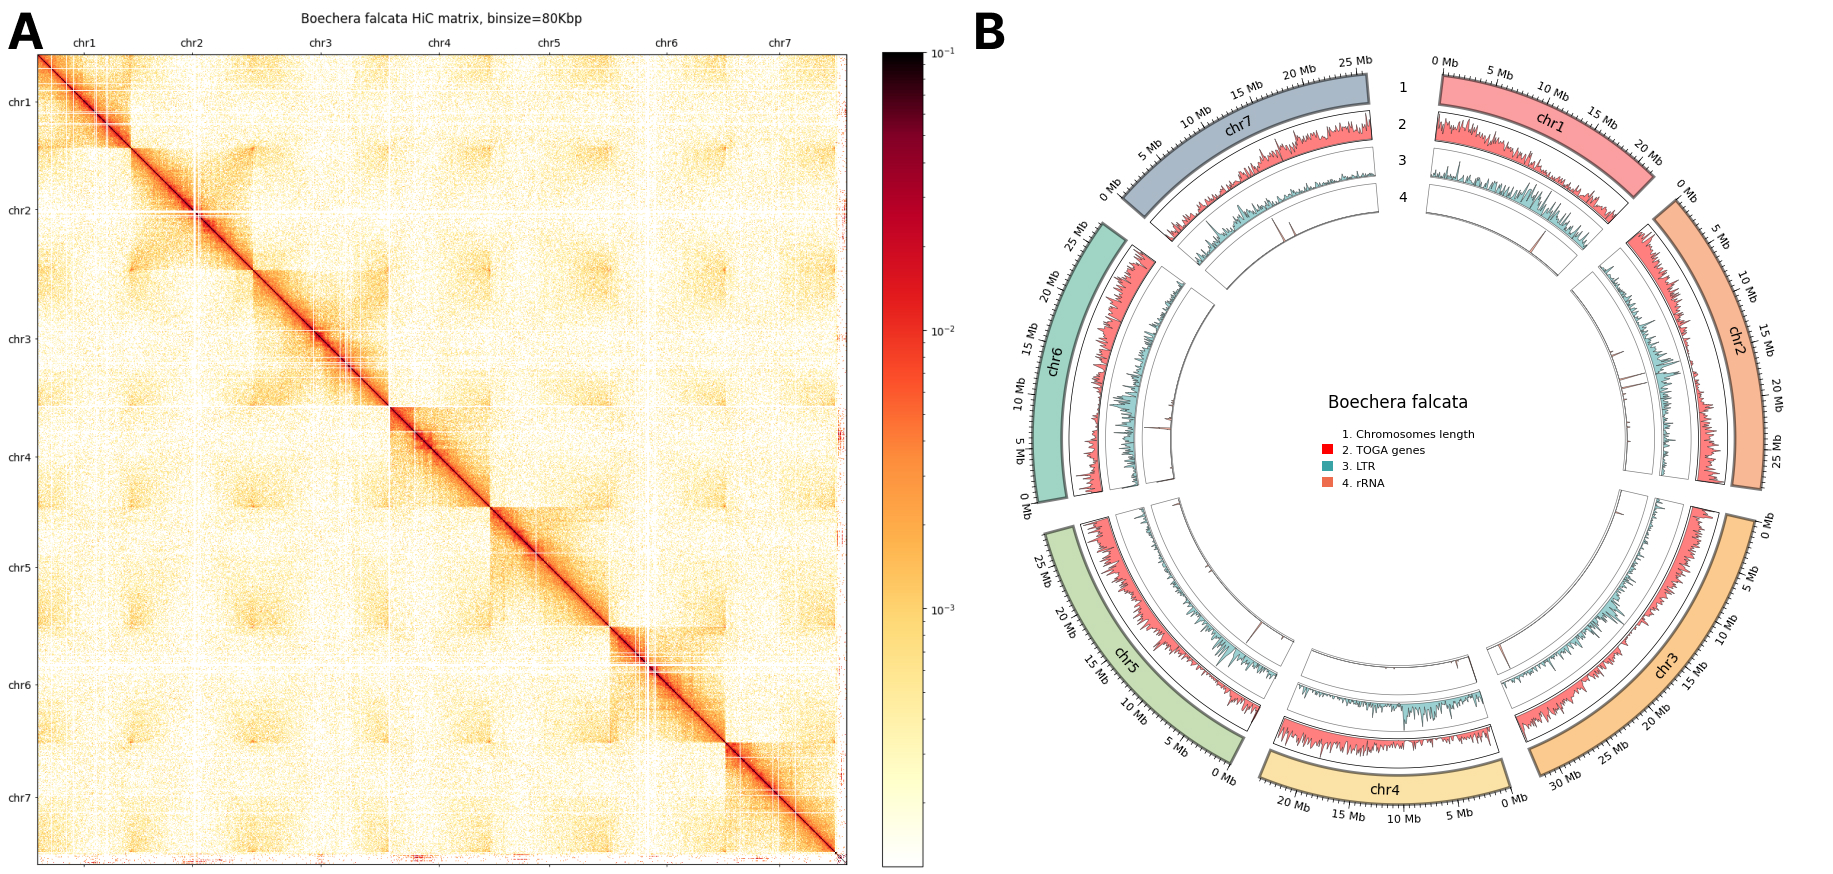
\includegraphics[width=\linewidth]{figures/heatmap_circos.jpg}
\caption{(A) Hi-C contact matrix of \textit{B. falcata} genome at 80Kbp resolution. The seven distinct chromosomes are clearly visible along the diagonal, indicating successful chromosome-level assembly. The intensity of red coloration represents the frequency of interactions between genomic regions, with darker red indicating higher interaction frequencies. (B) Circos plot of the genome assembly. HiC map was build with 80kbp bin size, circos plot includes (1) lengths of chromosomes, (2) frequency of genes in 100kbp bin size, (3) frequency of long tandem repeats in 100kbp bin size and (4) frequency of rRNA genes in the same bin size.}
\label{fig:hic-and-genome}
\end{figure}


\subsection{Analysis of Repetitive Elements}

The repeat masking analysis revealed that 38.46\% of the genome is made up of repetitive elements (Table \ref{tab:repeats_annotation}). Long Terminal Repeat (LTR) retrotransposons were the most common class of repeats, accounting for 19.76\% of the genome with 24,870 instances identified. DNA transposons represented the second most prevalent class, masking 6.23\% of the genome. Long Interspersed Nuclear Elements (LINEs) and Short Interspersed Nuclear Elements (SINEs) accounted for 2.39\% and 0.008\% of the genome, respectively. Other repetitive elements, including simple repeats, microsatellites, and RNA genes, comprised for a total of 0.65\% of the genome. Additionally, 8.82\% of the masked regions were classified as uncharacterized repetitive elements.

\begin{table*}[p]
\centering
\caption{Repeats revealed by RepeatMasker}
\begin{tableminipage}{\textwidth}
\begin{tabularx}{\textwidth}{@{}XXXX@{}}
\hline
\textbf{Class of repetitive element}       & \textbf{Total length} & \textbf{n of elements} & \textbf{\% of genome} \\
\hline
DNA                                        & 11783246              & 17307                  & 6.235                 \\
LINE                                       & 4527617               & 8007                   & 2.39                  \\
LTR                                        & 37373250              & 24870                  & 19.76                 \\
Other (Simple Repeat, Microsatellite, RNA) & 1221953               & 2131                   & 0.65                  \\
Penelope                                   & 24530                 & 259                    & 0.01                  \\
Rolling Circle                             & 1123003               & 2785                   & 0.59                  \\
SINE                                       & 15061                 & 234                    & 0.01                  \\
Unclassified                               & 16681735              & 47524                  & 8.82                  \\
\textbf{Total}                             & \textbf{72750395}     & \textbf{103117}        & \textbf{38.46}       \\
\hline
\end{tabularx}
  \label{tab:repeats_annotation}
\end{tableminipage}
\end{table*}

\subsection{Prediction of Protein-Coding Genes}

Homology-based prediction yielded a total of 27,516 protein-coding genes predicted. BUSCO analysis demonstrated completeness of annotation, with 99.2\% of the 4,596 BUSCO groups present and complete (Table \ref{tab:genes_annotation}).

\begin{table*}[p]
\centering
\caption{Homology-based gene prediction in \textit{Boechera falcata} genome }
\begin{tableminipage}{\textwidth}
\begin{tabularx}{\textwidth}{@{}XXXX@{}}
\hline
\textbf{Genes} & 27516                                                          \\
\textbf{Exons}          & 161159                                                         \\
\textbf{Introns}        & 130644                                                         \\
\textbf{mRNAs}          & 30516                                                          \\
\textbf{BUSCOs}         & C:99.2\% {[}S:78.83\%, D:20.37\%{]} F:0.13\%, M:0.67\%, N:4596 \\
\hline
\end{tabularx}
\label{tab:genes_annotation}
\end{tableminipage}
\end{table*}

\subsection{Comparative analysis of \textit{Boechera falcata} and \textit{Boechera stricta} genomes}

Comparative analysis of the \textit{Boechera falcata} and \textit{Boechera stricta} genomes revealed similarities in overall structure, as well as notable differences in assembly quality (Table \ref{tab:falcata_vs_stricta} ). Before the analysis, the genome of \textit{B. falcata} was oriented according to the \textit{B. stricta} genome. Both species possess 7 chromosomes and demonstrated highly comparable genome sizes of 189.36 Mb and 190.54 Mb and exhibited similar assembly contiguity metrics N50 of 27.20 Mb and 26.95 Mb for \textit{B. falcata} and \textit{B. stricta} correspondingly. BUSCO genome completeness scores are nearly identical for both species 98.8\% and 98.7\% for \textit{B. falcata} and \textit{B. stricta} accordingly, as well as gene counts, 27,516 in \textit{B. falcata}, 27,538 in \textit{B. stricta}. However, \textit{B. falcata} demonstrated higher assembly accuracy with higher Merqury QV (68.04 vs. 27.49) and Merfin QV (33.08 vs. 23.32) scores. Both genomes were assembled to chromosome level as diploid assemblies. Thus, combination of high structural similarity and improved accuracy of the \textit{B. falcata} genome assembly provides the basis for a detailed comparative analysis of its genome with other species of the genus \textit{Boechera}.

Analysis of structural variations between the \textit{Boechera falcata} and \textit{Boechera stricta} genomes revealed significant genomic rearrangements (Figure \ref{fig:falcata_vs_stricta} ). The comparison identified 294 syntenic regions, covering the majority of both genomes (Table \ref{tab:falcata_vs_stricta_synteny}). A total of 66 inversions were detected, spanning approximately 23.67 Mb in the reference genome (B. stricta) and 23.60 Mb in the query genome (B. falcata). These inversions represent substantial chromosomal rearrangements among the two species. Large regions of both genomes were found to be non-syntenic: 19.24 Mb are unique to \textit{B. stricta} and 18.36 Mb are unique to \textit{B. falcata}, indicating species-specific genomic content. Figure \ref{fig:falcata_vs_stricta} shows these structural variations on synteny plot (A) and dotplot (B).


\begin{table*}[p]
\centering
\caption{Comparison of genome characteristics of \textit{B.falcata} and \textit{B.stricta}} 
\begin{tableminipage}{\textwidth}
\begin{tabularx}{\textwidth}{@{}XXX@{}}
\hline
\textbf{Metric}    & \textit{\textbf{B.falcata}}                                    & \textit{\textbf{B.stricta} }                                    \\
\hline
Genome length (bp) & 189363209                                                      & 190536481                                                      \\
Chromosomes (x)    & 7                                                              & 7                                                              \\
N50 (bp)           & 27200968                                                       & 26945205                                                       \\
BUSCO genome       & C:98.8\% [D:3.0\%],F:0.2\%,M:1.0\%,n:4596          & C:98.7\% [D:3.0\%],F:0.3\%,M:1.0\%,n:4596          \\
Merqury QV         & 68.04                                   & 27.49                                                          \\
Merfin QV*         & 33.08                                                          & 23.32                                                          \\
Genes              & 27516                                                          & 27538                                                          \\
BUSCO annotation   & C:99.2\%[D:20.37\%],F:0.13\%,M:0.67\%,n:4596 & C:98,98\%[D:19.69\%],F:0.13\%,M:0.89\%,n:4596 \\
\hline
\end{tabularx}
\label{tab:falcata_vs_stricta} 
\end{tableminipage}
\end{table*}

\begin{table*}[p]
\centering
\caption{Synteny analysis characteristics}
\begin{tableminipage}{\textwidth}
\begin{tabularx}{\textwidth}{@{}XXXX@{}}
\hline
\textbf{Variation\_type} & \textbf{Count} & \textbf{Length\_ref (B.stricta)} & \textbf{Length\_qry (B.falcata)} \\
\hline
Syntenic regions         & 294            & 141724185                        & 141383384                        \\
Inversions               & 66             & 23669784                         & 23602144                         \\
Translocations           & 348            & 3730041                          & 3629426                          \\
Duplications (B.stricta) & 150            & 476406                           & -                                \\
Duplications (B.falcata) & 359            & -                                & 1366155                          \\
Not aligned (B.stricta)  & 801            & 19235167                         & -                                \\
Not aligned (B.falcata)  & 1030           & -                                & 18357653                         \\
\hline
\end{tabularx}
\label{tab:falcata_vs_stricta_synteny}
\end{tableminipage}
\end{table*}

\begin{figure}[t!]
\renewcommand{\familydefault}{\sfdefault}\normalfont
\centering
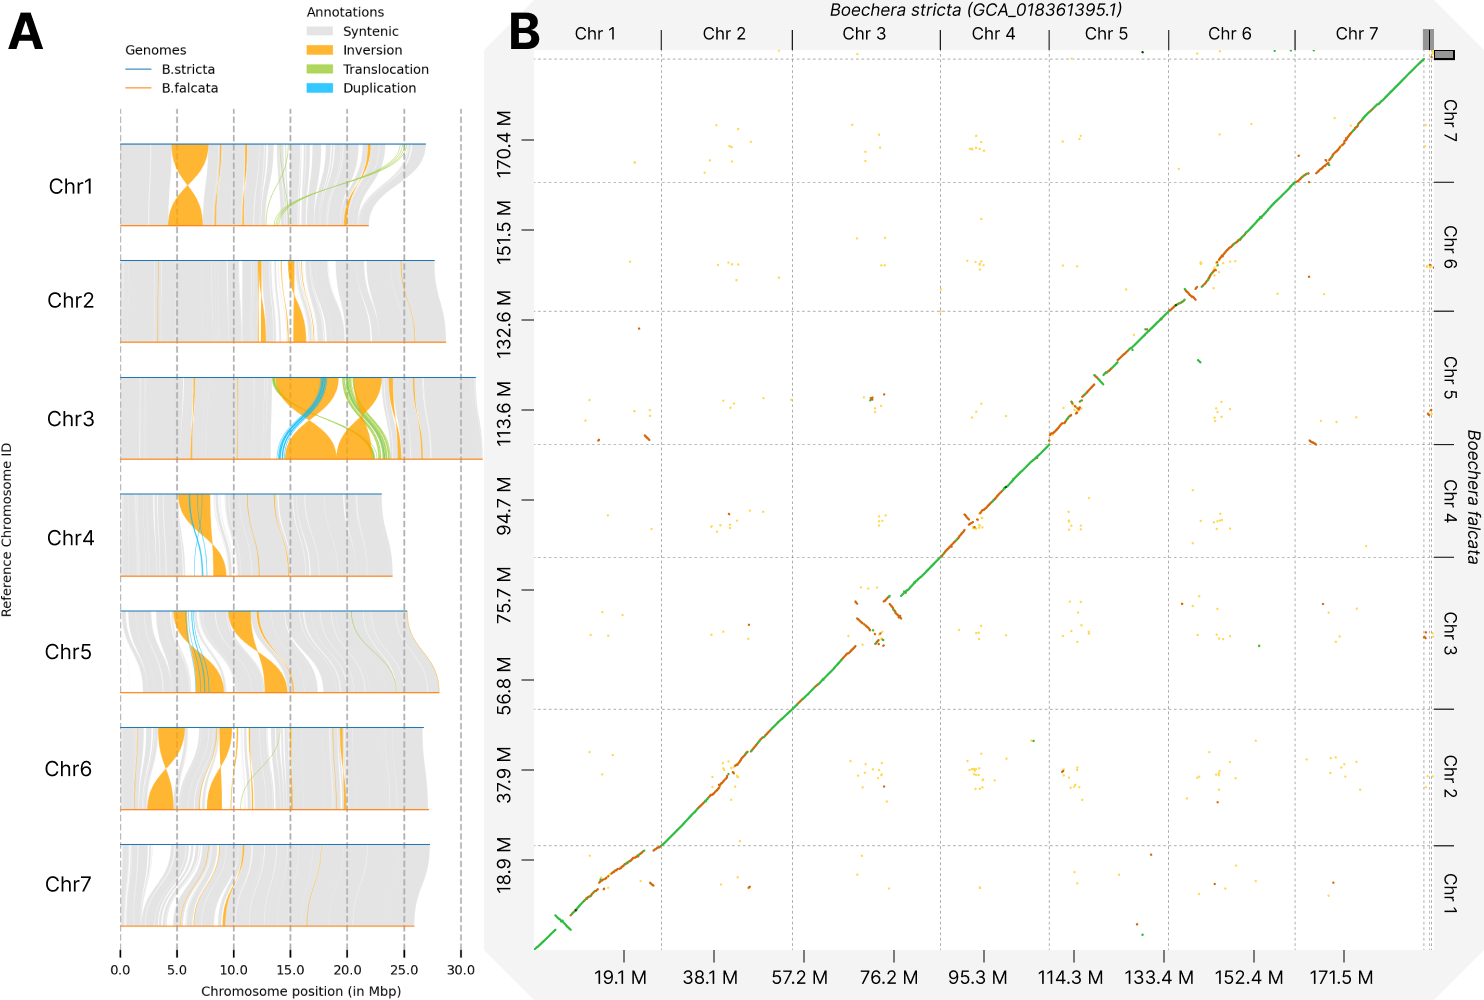
\includegraphics[width=\linewidth]{figures/Comparative stricta.png}
\caption{Illustration of the structural variations between \textit{Boechera stricta} and \textit{Boechera falcata} genomes. (A) chromosomal rearrangements, each chromosome of \textit{B. falcata} is aligned to \textit{B. stricta}. The orange regions represent inversions. Gray areas indicate syntenic regions. (B) Scatter plot of genome-wide comparison: chromosomes of \textit{B. stricta} on the x-axis and \textit{B. falcata} on the y-axis. Diagonal green lines represent syntenic regions with high sequence identity (\( >70\% \)), and yellow regions indicate areas with lower sequence identity (\( <70\% \)). Prominent large-scale inversions are visible, especially in chromosomes 1, 3, and 5 in (A) and corresponding off-diagonal patterns in (B). The dot plot highlights the overall conservation of chromosomal structure between the two species and also highlights significant inversions and areas of differing sequence identity across the genomes.}
\label{fig:falcata_vs_stricta} 
\end{figure}


\subsection{\textit{B. falcata} Falls into the Homozygous Sex Allele Clade on the \textit{APOLLO} Phylogenetic Tree}

The \textit{APOLLO} gene, encoding the NEN3 exonuclease, is an important apomixis-associated gene in \textit{Boechera} \citep{corral2013, brukhin2019}. The \textit{APOLLO} locus has previously been shown to have multiple alleles \citep{corral2013, kliver2018}. All studied apomictic plants carry at least one of the “apo” alleles, and the sexual accessions are homozygous for the “sex” alleles.
We decided to further explore the \textit{APOLLO} locus in the \textit{B. falcata} genome. The phylogenetic analysis of the \textit{APOLLO} gene revealed a clear division between two groups of \textit{Boechera} species, in accordance with their mode of reproduction (Figure 7), as was previously described \citep{kliver2018}. The tree shows two distinct clades within the \textit{Boechera} genus, with strong bootstrap support (100) for the split between these groups. One clade comprises apomictic \textit{Boechera spp.}, including apomictic \textit{Boechera} hybrid M4B, whose genome we assembled to chromosome scale previously (NCBI BioProject PRJNA774175), which forms a well-supported monophyletic group. The other clade comprises \textit{B. falcata}, \textit{B. arcuata}, \textit{B. retrofracta}, \textit{B. stricta} , and several \textit{Boechera spp.}, along with multiple \textit{B. spatifolia} accessions, which reproduce sexually. Notably, \textit{B. falcata} is positioned within this second clade, clustering closely with sexual \textit{B. arcuata} and \textit{Boechera spp.} (KF705572.1). This study demonstrates clear phylogenetic differentiation of the \textit{APOLLO} gene between the two groups of \textit{Boechera} species, with the \textit{B. falcata} group included in the clade that along with \textit{B. stricta} and other known sexual species.

\begin{figure}[t!]
\renewcommand{\familydefault}{\sfdefault}\normalfont
\centering
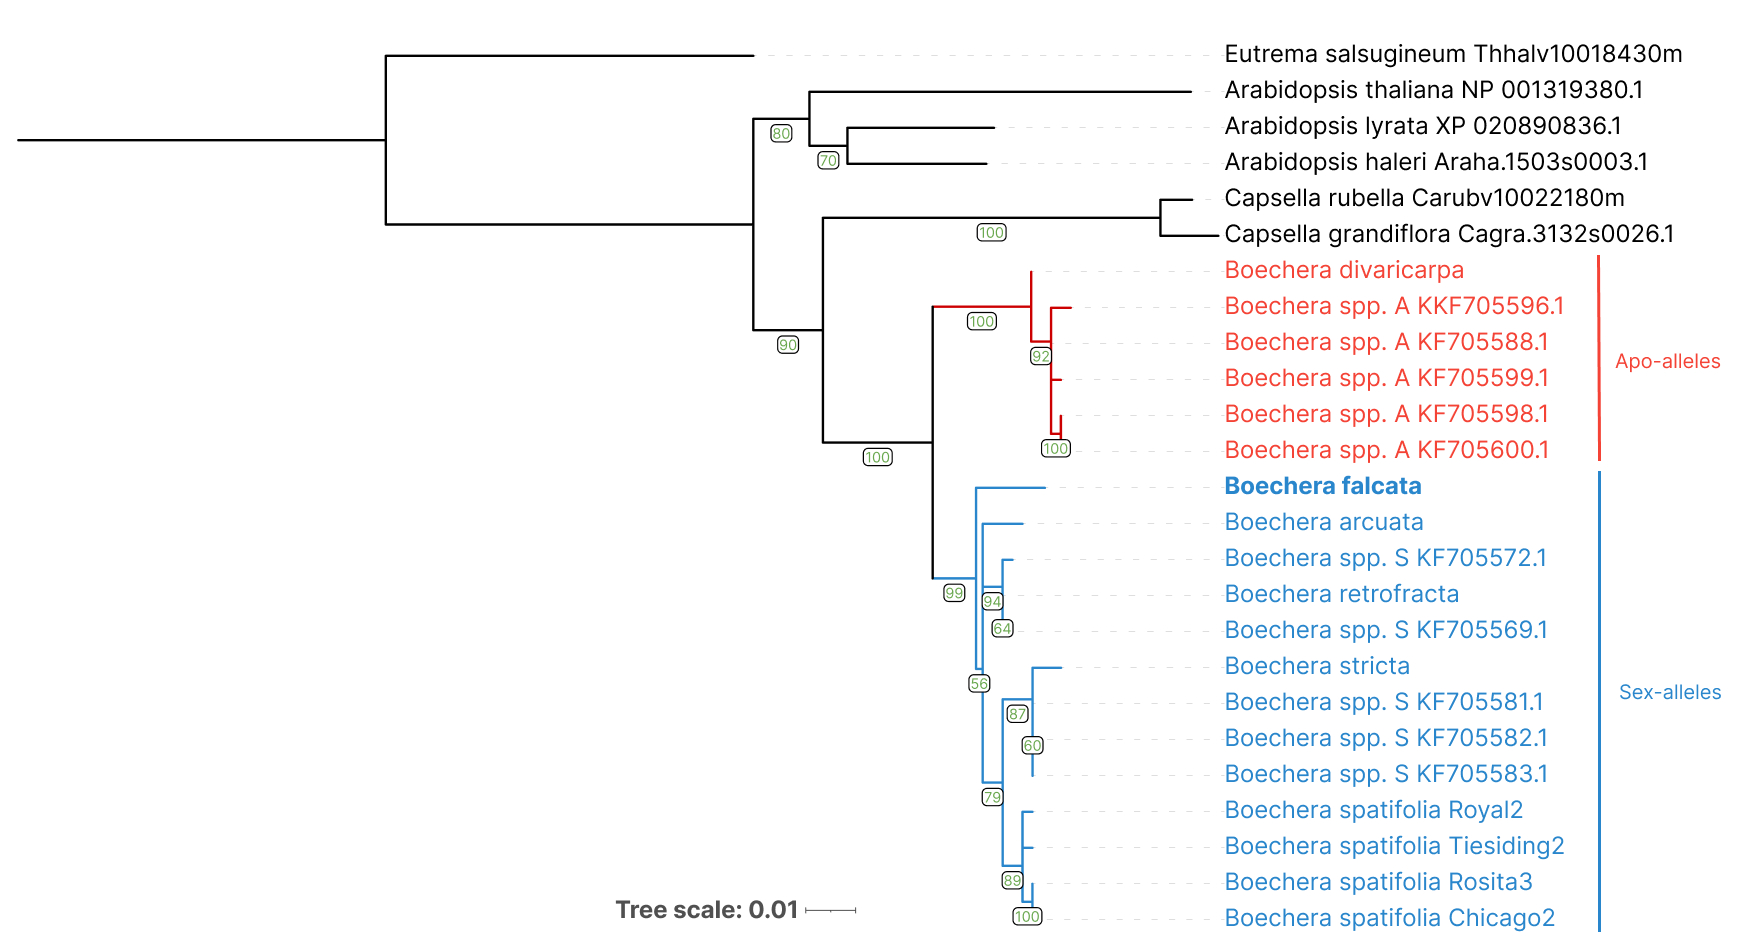
\includegraphics[width=\linewidth]{figures/apollo_phylogeny_bootstrap40_with_legend (3).jpg}
\caption{Phylogenetic tree of \textit{APOLLO} gene alleles in \textit{Boechera} and related species. Sequences of \textit{Eutrema salsugineum}, \textit{Arabidopsis thaliana}, \textit{A. lyrata}, \textit{A. haleri}, \textit{Capsella rubella}, and \textit{C. grandiflora} were used as outgroups. The two main clades within \textit{Boechera} are highlighted: apomictic species in red and sexual species in blue including \textit{B. falcata}. The numbers in the nodes represent bootstrap support values.}
\label{fig:apollo_tree}
\end{figure}

\subsection{Chloroplast and mitochondrial genome assembly and annotation}

To facilitate further evolutionary relationship study of non-model \textit{Boechera} species, phylogenetic researches, and species identifications we performed \textit{B. falcata} chloroplast and mitochondrial genomes assembly and annotation (Figure \ref{fig:chloroplast_and_mitochordria}). The entire size of the chloroplast genome is 155326 bp. 79 unique CDS, 30 tRNAs and 4 rRNA were identified in the chloroplast genome. Large single-copy (LSC) part and small single-copy (SSC) part of the chloroplast DNA occupy 84428 bp and 17952 bp respectively. GC contents is 36.41\%. All these indicators are consistent with those in the chloroplast genomes of other \textit{Boechera} species as shown in Table \ref{tab:chloroplast_compare}.

Length of the mitochondrial DNA in \textit{B. falcata} is 292 083 bp and GC content is 44.90\% (Figure \ref{fig:chloroplast_and_mitochordria}). Comparative data on the mitochondrial genome size and GC content in \textit{B. falcata}, \textit{B. stricta}, and \textit{A. thaliana} are shown in table \ref{tab:mito_compare}. Table \ref{tab:mito_genes} indicates the type and functions of the genes identified in mitochondrial DNA of \textit{B. falcata}, \textit{B. stricta}, and \textit{A. thaliana}. All in all 33 protein-coding genes, 17 tRNAs and 3 rRNAs were annotated in the mitochondrial genome of \textit{B. falcata}.


\begin{figure}[t!]
\renewcommand{\familydefault}{\sfdefault}\normalfont
\centering
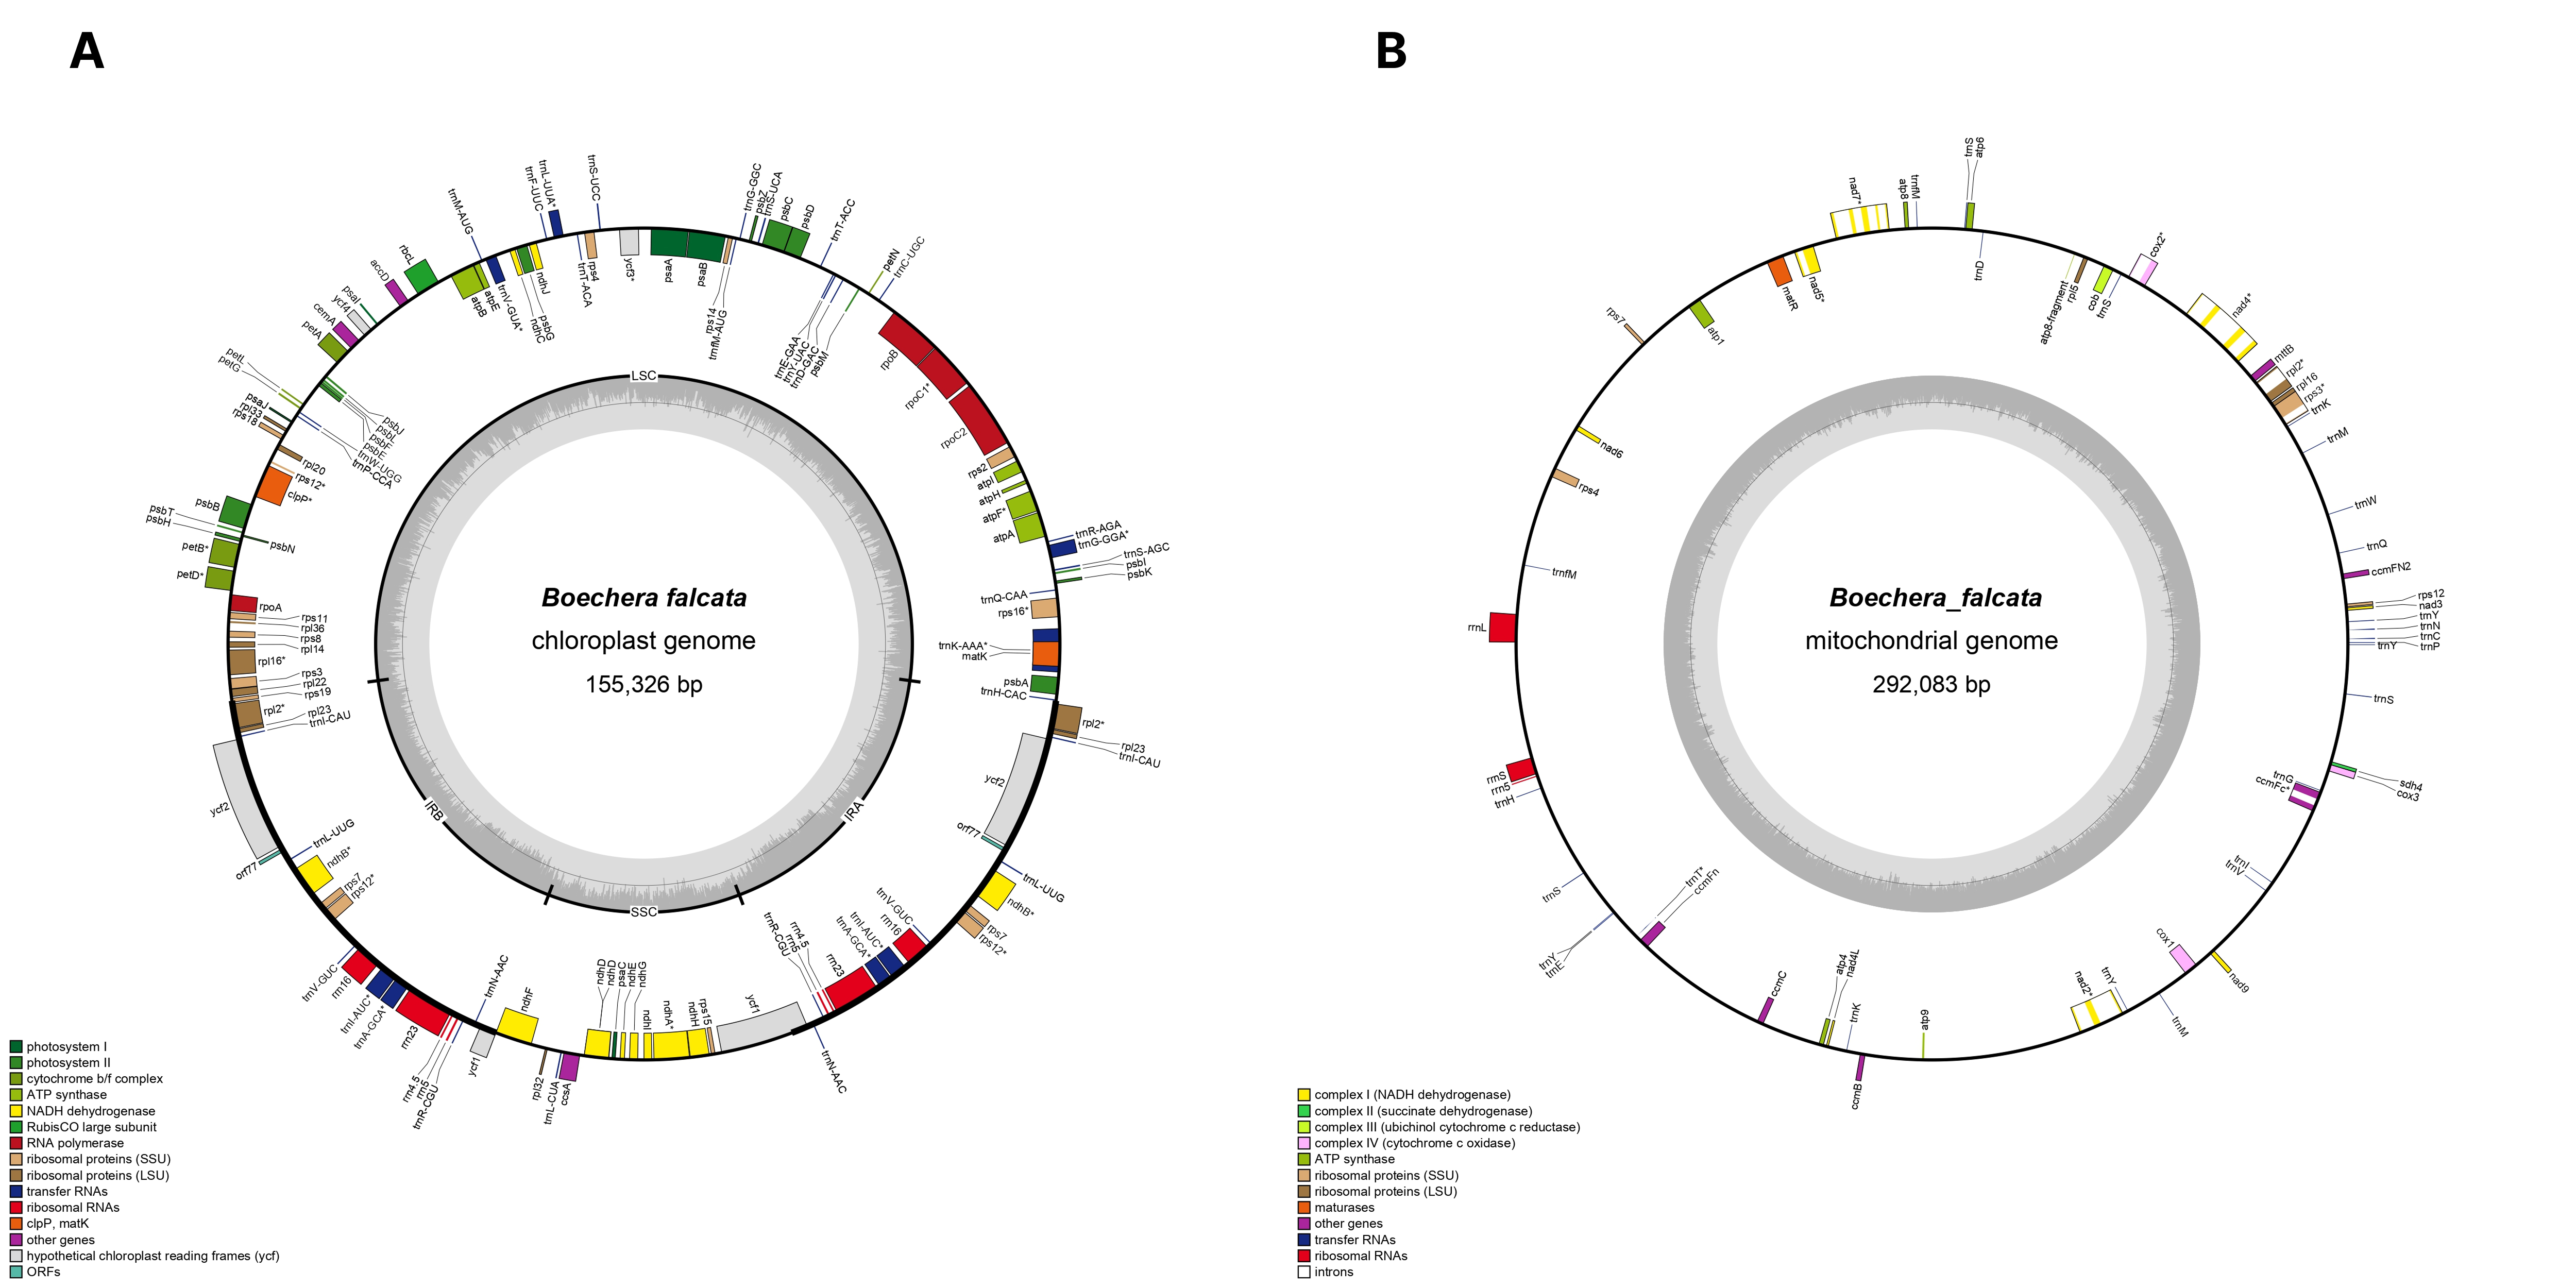
\includegraphics[width=\linewidth]{figures/boechera_organeles_circos.jpg}
\caption{Circular representation of \textit{B. falcata} (A) chloroplast genome and (B) mitochondrial genome. Gray circle inside shows \% of GC content.}
\label{fig:chloroplast_and_mitochordria}
\end{figure}


\begin{table*}[p]
\centering
\caption{Comparison of several \textit{Boechera} species chloroplast genomes }
\begin{tableminipage}{\textwidth}
\begin{tabularx}{\textwidth}{@{}l l XXXXXXXXXXX@{}}
\hline
\textbf{Species name}           & \textbf{RefSeq ID} & \textbf{Genome size (bp)} & \textbf{LSC Len (bp)} & \textbf{SSC Len (bp)} & \textbf{IR Len (bp)} & \textbf{CDS} & \textbf{tRNAs} & \textbf{rRNAs} & \textbf{Total GC(\%)} & \textbf{LSC GC(\%)} & \textbf{SSC GC(\%)} & \textbf{IR GC(\%)} \\
\hline
\textit{Boechera falcata}       & chloroplast                      & 155326                    & 84428                    & 17952                    & 26473                   & 79           & 30             & 4              & 36.41                        & 34.20               & 29.42               & 42.33              \\
\textit{Boechera suffrutescens} & NC\_049600.1                     & 155114                    & 84285                    & 17915                    & 26457                   & 79           & 30             & 4              & 36.43                        & 34.18               & 29.52               & 42.36              \\
\textit{Boechera stricta}        & NC\_049599.1                     & 155033                    & 84237                    & 17884                    & 26456                   & 79           & 30             & 4              & 36.39                        & 34.15               & 29.38               & 42.33              \\
\textit{Boechera pulchra}       & NC\_049598.1                     & 155348                    & 84483                    & 17951                    & 26457                   & 79           & 30             & 4              & 36.42                        & 34.17               & 29.49               & 42.37              \\
\textit{Boechera puberula}      & NC\_049597.1                     & 155011                    & 84189                    & 17928                    & 26447                   & 79           & 30             & 4              & 36.48                        & 34.26               & 29.63               & 42.35              \\
\textit{Boechera laevigata}     & NC\_049596.1                     & 155083                    & 84266                    & 17891                    & 26463                   & 79           & 30             & 4              & 36.45                        & 34.22               & 29.48               & 42.33              \\
\textit{Boechera davidsonii}    & NC\_049594.1                     & 154935                    & 84107                    & 17914                    & 26457                   & 79           & 30             & 4              & 36.46                        & 34.24               & 29.57               & 42.33              \\
\textit{Boechera breweri}       & NC\_049593.1                     & 155147                    & 84347                    & 17886                    & 26457                   & 79           & 30             & 4              & 36.44                        & 34.21               & 29.56               & 42.33              \\
\hline
\end{tabularx}
\label{tab:chloroplast_compare}
\end{tableminipage}
\end{table*}

\begin{table*}[p]
\centering
\caption{Comparative data on mitochondrial genome size and GC content in \textit{B. falcata}, \textit{B. stricta} , and \textit{A. thaliana}}
\begin{tableminipage}{\textwidth}
\begin{tabularx}{\textwidth}{@{}XXXX@{}}
\hline
\textbf{Species name}         & \textbf{RefSeq accession number} & \textbf{Genome size (bp)} & \textbf{GC content \%} \\
\hline
\textit{Boechera falcata}     & mithochondrion                   & 292083                    & 44.90                  \\
\textit{Boechera stricta}      & NC\_042143.1                     & 271601                    & 44.93                  \\
\textit{Arabidopsis thaliana} & NC\_037304.1                     & 367808                    & 44.79                 \\
\hline
\end{tabularx}
\label{tab:mito_compare}
\end{tableminipage}
\end{table*}

\begin{table*}[p]
\centering
\caption{Characteristics of the genes identified in mitochondrial DNA of \textit{B. falcata}, \textit{B. stricta}, and \textit{A. thaliana}}
\begin{tableminipage}{\textwidth}
\begin{tabularx}{\textwidth}{@{}XXXX@{}}
\hline
\textbf{Group of genes}          & \textit{\textbf{Boechera falcata}}                                                                    & \textit{\textbf{Boechera stricta} }                                                        & \textit{\textbf{Arabidopsis thaliana}}                                                    \\
\hline
ATP synthase                     & atp1, atp4, atp6, atp8, atp9                                                                          & atp1, atp4, atp6, atp8, atp9                                                              & atp1, atp4, atp6, atp8, atp9                                                              \\
Cytochrome c biogenesis          & ccmB, ccmC, ccmFc, ccmFn, ccmFN2                                                                      & ccmB, ccmC, ccmFc, ccmFn                                                                  & ccmB, ccmC, ccmFC, ccmFN1, ccmFN2                                                         \\
Ubiquinol cytochrome c reductase & cob                                                                                                   & cob                                                                                       & cob                                                                                       \\
Cytochrome c oxidase             & cox1, cox2, cox3                                                                                      & cox1, cox2, cox3                                                                          & cox1, cox2, cox3                                                                          \\
Maturases                        & matR                                                                                                  & matR                                                                                      & matR                                                                                      \\
Transport membrane protein       & mttB                                                                                                  & mttB                                                                                      & mttB                                                                                      \\
NADH dehydrogenase               & nad1, nad2, nad3, nad4, nad4L, nad5, nad6, nad7, nad9                                                 & nad1, nad2, nad3, nad4, nad4L, nad5, nad6, nad7, nad9                                     & nad1, nad2, nad3, nad4, nad4L, nad5, nad6, nad7, nad9                                     \\
Large subunit of ribosome        & rpl2, rpl5, rpl16                                                                                     & rpl2, rpl5, rpl16                                                                         & rpl2, rpl5, rpl16                                                                         \\
Small subunit of ribosome        & rps3, rps4, rps7, rps12                                                                               & rps3, rps4, rps12                                                                         & rps3, rps4, rps7, rps12                                                                   \\
Succinate dehydrogenase          & sdh4                                                                                                  & sdh4                                                                                      & -                                                                                         \\
Ribosomal RNAs                   & rrn5, rrn18, rrn26                                                                                    & rrn5, rrn18, rrn26                                                                        & rrn5, rrn18, rrn26                                                                        \\
Transfer RNAs                    & trnC, trnD, trnE, trnG, trnH, trnI, trnK, trnM, trnN, trnP, trnQ, trnS, trnT, trnV, trnW, trnY, trnfM & trnC, trnD, trnE, trnG, trnH, trnI, trnK, trnM, trnN, trnP, trnQ, trnS, trnW, trnY, trnfM & trnC, trnD, trnE, trnG, trnH, trnI, trnK, trnM, trnN, trnP, trnQ, trnS, trnW, trnY, trnfM \\
\hline
\end{tabularx}
\label{tab:mito_genes}
\end{tableminipage}
\end{table*}


\subsection{Phylogeny of \textit{B. falcata} and Its Relationship with Other \textit{Boechera} and Brassicaceae species}

A phylogenetic tree of Brassicaceae constructed based on 47 chloroplast genes (\textbf{Suppl. Figure 3}, \textit{B. falcata} highlighted in bold) confirms the monophyly of the sampled \textit{Boechera} species within the tribe Boechereae. Notably, \textit{B. falcata} , the first representative of the genus from Eurasia to be included in such a chloroplast genome analysis, is deeply nested within the single major \textit{Boechera} clade recovered, which otherwise consists entirely of North American species.

The placement of \textit{B. falcata} firmly within the clade of predominantly North American \textit{Boechera} species, rather than in a basal position or as a sister group to North American taxa, suggests a North American origin for \textit{B. falcata}. The fact that this Eurasian species falls within the only identified \textit{Boechera} lineage, rather than forming a distinct Eurasian clade, further supports this interpretation. This phylogenetic position implies that \textit{B. falcata}'s maternal lineage originated in North America and subsequently dispersed to North-East of Eurasia, likely across Beringia during periods when a land bridge was present, or possibly via long-distance dispersal. This finding aligns with previous phylogeographic studies based on fewer chloroplast markers, which also indicated a North American center of diversity for \textit{Boechera} \citep{dobevs2004extensive, dobevs2004intraspecific, kiefer2009phylogeographic}. This chloroplast based phylogeny provides evidence for \textit{Boechera} intrageneric intercontinental exchange, which is an example of East Asian/North American floristic disjunction.

The combination of Angiosperms353 and Brassicaceae764 probe sets revealed a comprehensive evolutionary relationship within the Boechereae tribe (Figure \ref{fig:full_boechera_tree}). The tree strongly supports the deep divergence between \textit{Boechera} sensu stricto and the non-Boechera Boechereae (NBB) clade, consistent with previous studies \citep{hay2023}. Within \textit{Boechera} s.s., we observed three main core groups (Core \textit{Boechera} I, II, and III). \textit{B. falcata} , the focus of our study, is positioned within the Core \textit{Boechera} III, sister to what \citep{hay2023} called the Boreal clade. This placement provides new insights into the phylogenetic relationships of \textit{B. falcata} within the broader \textit{Boechera} genus. The tree topology and strong bootstrap support of many nodes demonstrate the power of combining these probe sets for resolving relationships within this complex group.

\begin{figure}[t!]
\renewcommand{\familydefault}{\sfdefault}\normalfont
\centering
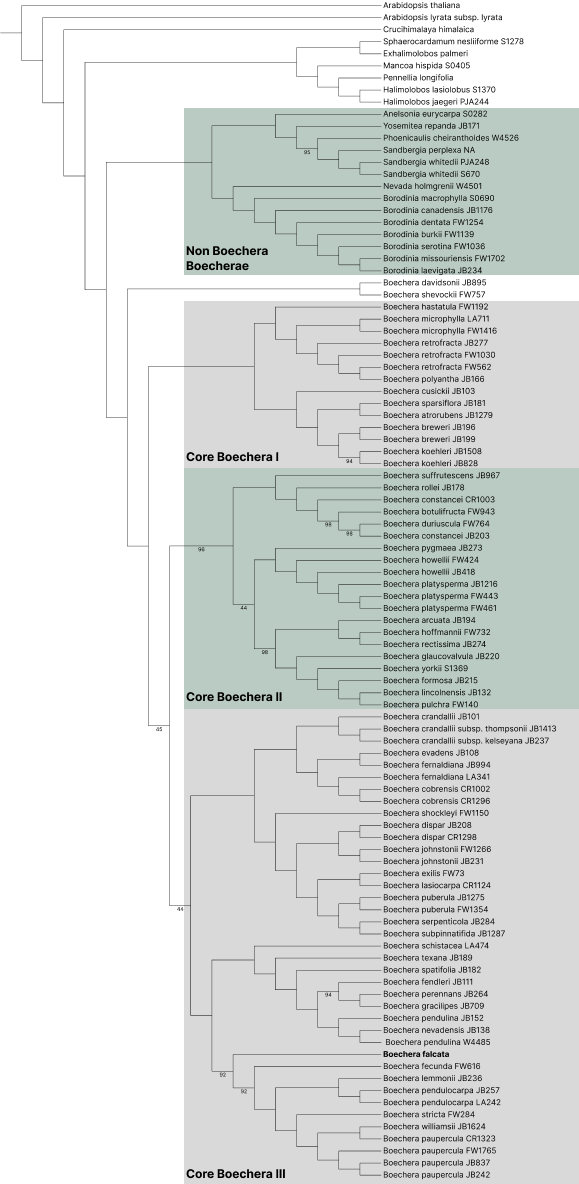
\includegraphics[width=\linewidth]{figures/Boechera_tree.png}
\caption{Phylogenetic tree of Boechereae and related species based on combined Angiosperms353 and Brassicaceae764 probe sets. The tree is rooted with outgroup species including \textit{Arabidopsis thaliana} and \textit{Schrenkiella parvula}. Major clades are highlighted. \textit{Boechera falcata} is indicated in bold. Numbers at nodes represent bootstrap support values <100.}
\label{fig:full_boechera_tree}
\end{figure}


\section{Conclusion}

To conclude, we present a high-quality genome assembly of the only \textit{Boechera} species native to Eurasia, (the Far Eastern \textit{B. falcata} ) to the chromosome level, as well as an assembly of chloroplast and mitochondrial DNA. The highly homozygous genome, the presence of only sex alleles of the \textit{APOLLO} gene, and previously obtained cytoembryological data suggest that this species reproduces only sexually. It likely came to the Eurasian continent from North America across the Bering Land Bridge during the Pleistocene glacial maxima. In terms of genome morphology, structure and size, as well as chromosome arrangement and organelle DNA organization, this species is quite close to its North American sexual relatives from the Boechereae tribe. Using molecular probes, it was possible to confirm the placement of \textit{B. falcata} within tribe Boechereae, namely in the Core \textit{Boechera} III group. A phylogenetic tree constructed based on the chloroplast DNA confirmed the phylogenetic analysis using molecular probes. Within our sampling for the chloroplast DNA phylogeny, \textit{B. falcata} appears related to North-American \textit{Boechera}. Finally, the availability of the genome of the only Eurasian \textit{Boechera} species will help studies of the evolution and phylogeny of Brassicaceae species, as well as apomixis researchers to unravel the complex hybridization events that form \textit{Boechera} apomicts.

\section{Data availability}


Sequencing data and genome assemblies are available through NCBI BioProject PRJNA1134229. Repeats and gene annotation for both \textit{B. falcata} and \textit{B. stricta} can be found on GitHub at \url{https://github.com/zilov/boechera_falcata_article}. Supplimentary data attached to the article.


\section{Acknowledgments}

The work was carried out within the framework of the state assignment of the Komarov Botanical Institute RAS No. 124013100862-0 “Polyvariance of morphogenetic programs for the development of plant reproductive structures, regulation of morphological processes in vivo and in vitro” (2024-2028) and RFBR grant No. 20-54-46002 “Phylogenetic and functional analysis of genes associated with apomixis in representatives of the \textit{Boechera} genus” to VB. This work was further supported by the Czech Science Foundation (project 24-11371S to TM). Seeds and photographs of \textit{B. falcata} plants were kindly provided by Dr. N.V. Sinelnikova from the Institute of Biological Problems of the North, Far Eastern Branch RAS.

\section{Funding}

The work was carried out within the framework of the state assignment of the Komarov Botanical Institute RAS No. 124013100862-0 “Polyvariance of morphogenetic programs for the development of plant reproductive structures, regulation of morphological processes in vivo and in vitro” (2024-2028) and RFBR grant No. 20-54-46002 “Phylogenetic and functional analysis of genes associated with apomixis in representatives of the \textit{Boechera} genus” to VB. This work was further supported by the Czech Science Foundation (project 24-11371S to TM).

\section{Conflicts of interest}
The author(s) declare no conflicts of interest.

\bibliography{example-bibliography}

\end{document} 